\documentclass[aspectratio=169, 10pt]{beamer}
\usepackage[utf8]{inputenc}
\usepackage[T1]{fontenc}
\usepackage{tikz}
\usepackage{booktabs}
\usepackage{graphicx}
\usepackage{tcolorbox}
\usepackage{colortbl}
\usepackage{amsmath}
\usepackage{xcolor}
\usetikzlibrary{calc, positioning, shadows, patterns, decorations.pathmorphing}

% ==========================================
% VIBRANT ORIGINAL DESIGN: MIDNIGHT & AMBER
% ==========================================
\definecolor{Midnight}{HTML}{0F172A}
\definecolor{VibrantAmber}{HTML}{F59E0B}
\definecolor{SoftMint}{HTML}{ECFDF5}
\definecolor{EmeraldEdge}{HTML}{10B981}
\definecolor{SlateText}{HTML}{1E293B}
\definecolor{RoseGold}{HTML}{FB7185}

\setbeamercolor{background canvas}{bg=white}
\setbeamercolor{normal text}{fg=SlateText}
\setbeamercolor{itemize item}{fg=VibrantAmber}
\setbeamertemplate{navigation symbols}{}

% CUSTOM DOODLE: HEARTBEAT
\newcommand{\heartbeatdoodle}[1]{
    \begin{tikzpicture}[#1]
        \draw[RoseGold, line width=1.5pt, cap=round, join=round] 
        (0,0) -- (0.2,0) -- (0.3,0.5) -- (0.4,-0.5) -- (0.5,1.2) -- (0.6,-0.8) -- (0.7,0) -- (1,0);
    \end{tikzpicture}
}

% CUSTOM DOODLE: DATA WAVE
\newcommand{\datawavedoodle}[1]{
    \begin{tikzpicture}[#1]
        \draw[EmeraldEdge, line width=1pt, opacity=0.4] 
        plot [smooth, tension=1] coordinates {(0,0) (0.5,0.3) (1,-0.2) (1.5,0.5) (2,0)};
    \end{tikzpicture}
}

% Header Template
\setbeamertemplate{frametitle}{
    \nointerlineskip
    \begin{beamercolorbox}[wd=\paperwidth,ht=1.4cm,dp=0.4cm]{frametitle}
        \begin{tikzpicture}[remember picture, overlay]
            \fill[Midnight] (current page.north west) rectangle ($(current page.north east) - (0, 1.4)$);
            \fill[VibrantAmber] ($(current page.north east) - (2.5, 0)$) -- ($(current page.north east) - (1.5, 1.4)$) -- (current page.north east) -- cycle;
            \draw[VibrantAmber, line width=3pt] ($(current page.north west) + (0, -1.4)$) -- ($(current page.north east) + (0, -1.4)$);
            \node[anchor=west, white, font=\Large\bfseries] at ($(current page.north west) + (0.6, -0.7)$) {\insertframetitle};
            \node[anchor=east] at ($(current page.north east) + (-0.2, -0.7)$) {\heartbeatdoodle{scale=0.4}};
        \end{tikzpicture}
    \end{beamercolorbox}
    \vspace{0.4cm}
}

% Footer Template
\setbeamertemplate{footline}{
    \begin{tikzpicture}[remember picture, overlay]
        \fill[Midnight!5] (current page.south west) rectangle (current page.south east);
        \draw[Midnight!20, line width=0.5pt] (current page.south west) -- (current page.south east);
        \node[anchor=west, Midnight!60, font=\tiny] at ($(current page.south west) + (0.3, 0.25)$) {\textbf{Applied Project} \textbar\ Group Members};
        \node[anchor=east, Midnight, font=\tiny\bfseries] at ($(current page.south east) + (-0.3, 0.25)$) {\insertframenumber};
    \end{tikzpicture}
    \vspace{0.5cm}
}

% Command for Vertical Metric Tables
\newcommand{\metricwidget}[5]{
    \begin{tcolorbox}[colback=white, colframe=Midnight, boxrule=1pt, arc=0pt, 
        title=\textbf{Performance Snapshot}, coltitle=white, colbacktitle=Midnight]
        \renewcommand{\arraystretch}{1.4}
        \small
        \begin{tabular}{ll}
            \textbf{Metric} & \textbf{Value} \\ \midrule
            \textbf{MAE} & \textcolor{RoseGold}{\textbf{#2}} \\
            \textbf{RMSE} & #3 \\
            \textbf{MAPE} & \textbf{#4\%} \\
            \textbf{R$^2$ Score} & \textbf{#5} \\
        \end{tabular}
    \end{tcolorbox}
}

% Chapter Page
\newcommand{\newchapter}[2]{
    \begin{frame}[plain]
        \begin{tikzpicture}[remember picture, overlay]
            \fill[Midnight] (current page.north west) rectangle (current page.south east);
            \node[anchor=center, VibrantAmber, font=\huge\bfseries] at ($(current page.center) + (0, 0.6)$) {PART #1};
            \node[anchor=center, white, font=\LARGE\bfseries] at ($(current page.center) + (0, -0.4)$) {#2};
            \draw[EmeraldEdge, line width=4pt] ($(current page.center) + (-3, 0.1)$) -- ($(current page.center) + (3, 0.1)$);
        \end{tikzpicture}
    \end{frame}
}

% Image Slide Macro
\newcommand{\imageslide}[3]{
    \begin{frame}{#1}
        \centering
        \includegraphics[width=0.9\textwidth, height=0.7\textheight, keepaspectratio]{#2}
        \vspace{0.2cm}
        \begin{tcolorbox}[colback=Midnight!5, colframe=Midnight, boxrule=0.5pt, sharp corners]
            \centering \small \textit{#3}
        \end{tcolorbox}
    \end{frame}
}

\begin{document}

% 1: TITLE
\begin{frame}[plain]
    \begin{tikzpicture}[remember picture, overlay]
        \fill[Midnight] (current page.north west) rectangle (current page.south east);
        \node[anchor=center, white, font=\huge\bfseries, align=center] at ($(current page.center) + (0, 1.5)$) {Applied Forecasting:\\ Stress Prediction Pipeline};
        \node[anchor=center, VibrantAmber, font=\Large] at ($(current page.center) + (0, 0.2)$) {13-Model Benchmarking \& Analytical Validation};
        \draw[EmeraldEdge, line width=2pt] ($(current page.center) + (-5, 0.8)$) -- ($(current page.center) + (5, 0.8)$);
        \node[anchor=south, white, align=center] at ($(current page.south) + (0, 1)$) {
            \small Nilesh Mori \textbar\ Harsh Maheriya \textbar\ Dhanush Pillai \textbar\ Megh Jagtap \\
            \small \textcolor{VibrantAmber}{May 10, 2026 \textbar\ DA-IICT}
        };
    \end{tikzpicture}
\end{frame}

\newchapter{I}{Introduction \& Data Audit}
\begin{frame}{Problem Statement: Proactive Stress Monitoring}
    \begin{itemize}
        \item \textbf{Reactive:} Detecting stress \textbf{after} onset.
        \item \textbf{Proactive:} Forecasting stress intensity \textbf{before} it peaks.
        \item \textbf{Goal:} Achieve <9\% MAPE using historical physiological context.
    \end{itemize}
\end{frame}

\imageslide{Subject S2 Baseline}{EDA_Graphs/01_S2_Proper_Timeline.png}{High-resolution synchronization of multimodal sensors.}
\imageslide{Stationarity Audit}{EDA_Graphs/05_Differenced_Signal_Timeline.png}{Proof of stationarity ($p \approx 0.000$) after first-order differencing.}
\imageslide{Lag Correlation Diagnostics}{EDA_Graphs/06_Stationary_Lag_Diagnostics.png}{ACF/PACF patterns confirming model orders p=2 and q=3.}

\newchapter{II}{Pipeline Engineering Fixes}
\begin{frame}{Fixing Critical Failures}
    \begin{enumerate}
        \item \textbf{Binary Box Fix:} Converted discrete labels to smooth intensity scores.
        \item \textbf{Leakage Protection:} Implemented strict $t-1$ lag for all sensor predictors.
        \item \textbf{Walk-Forward Protocol:} Used rolling forecasts to simulate real-world monitoring.
    \end{enumerate}
\end{frame}

\newchapter{III}{Model Deep-Dive \& Results}

\begin{frame}{Model 1: Naive Baseline}
    \textbf{\textcolor{VibrantAmber}{Theory:}} $\hat{y}_{t+1} = y_t$
    \begin{columns}
        \begin{column}{0.65\textwidth} 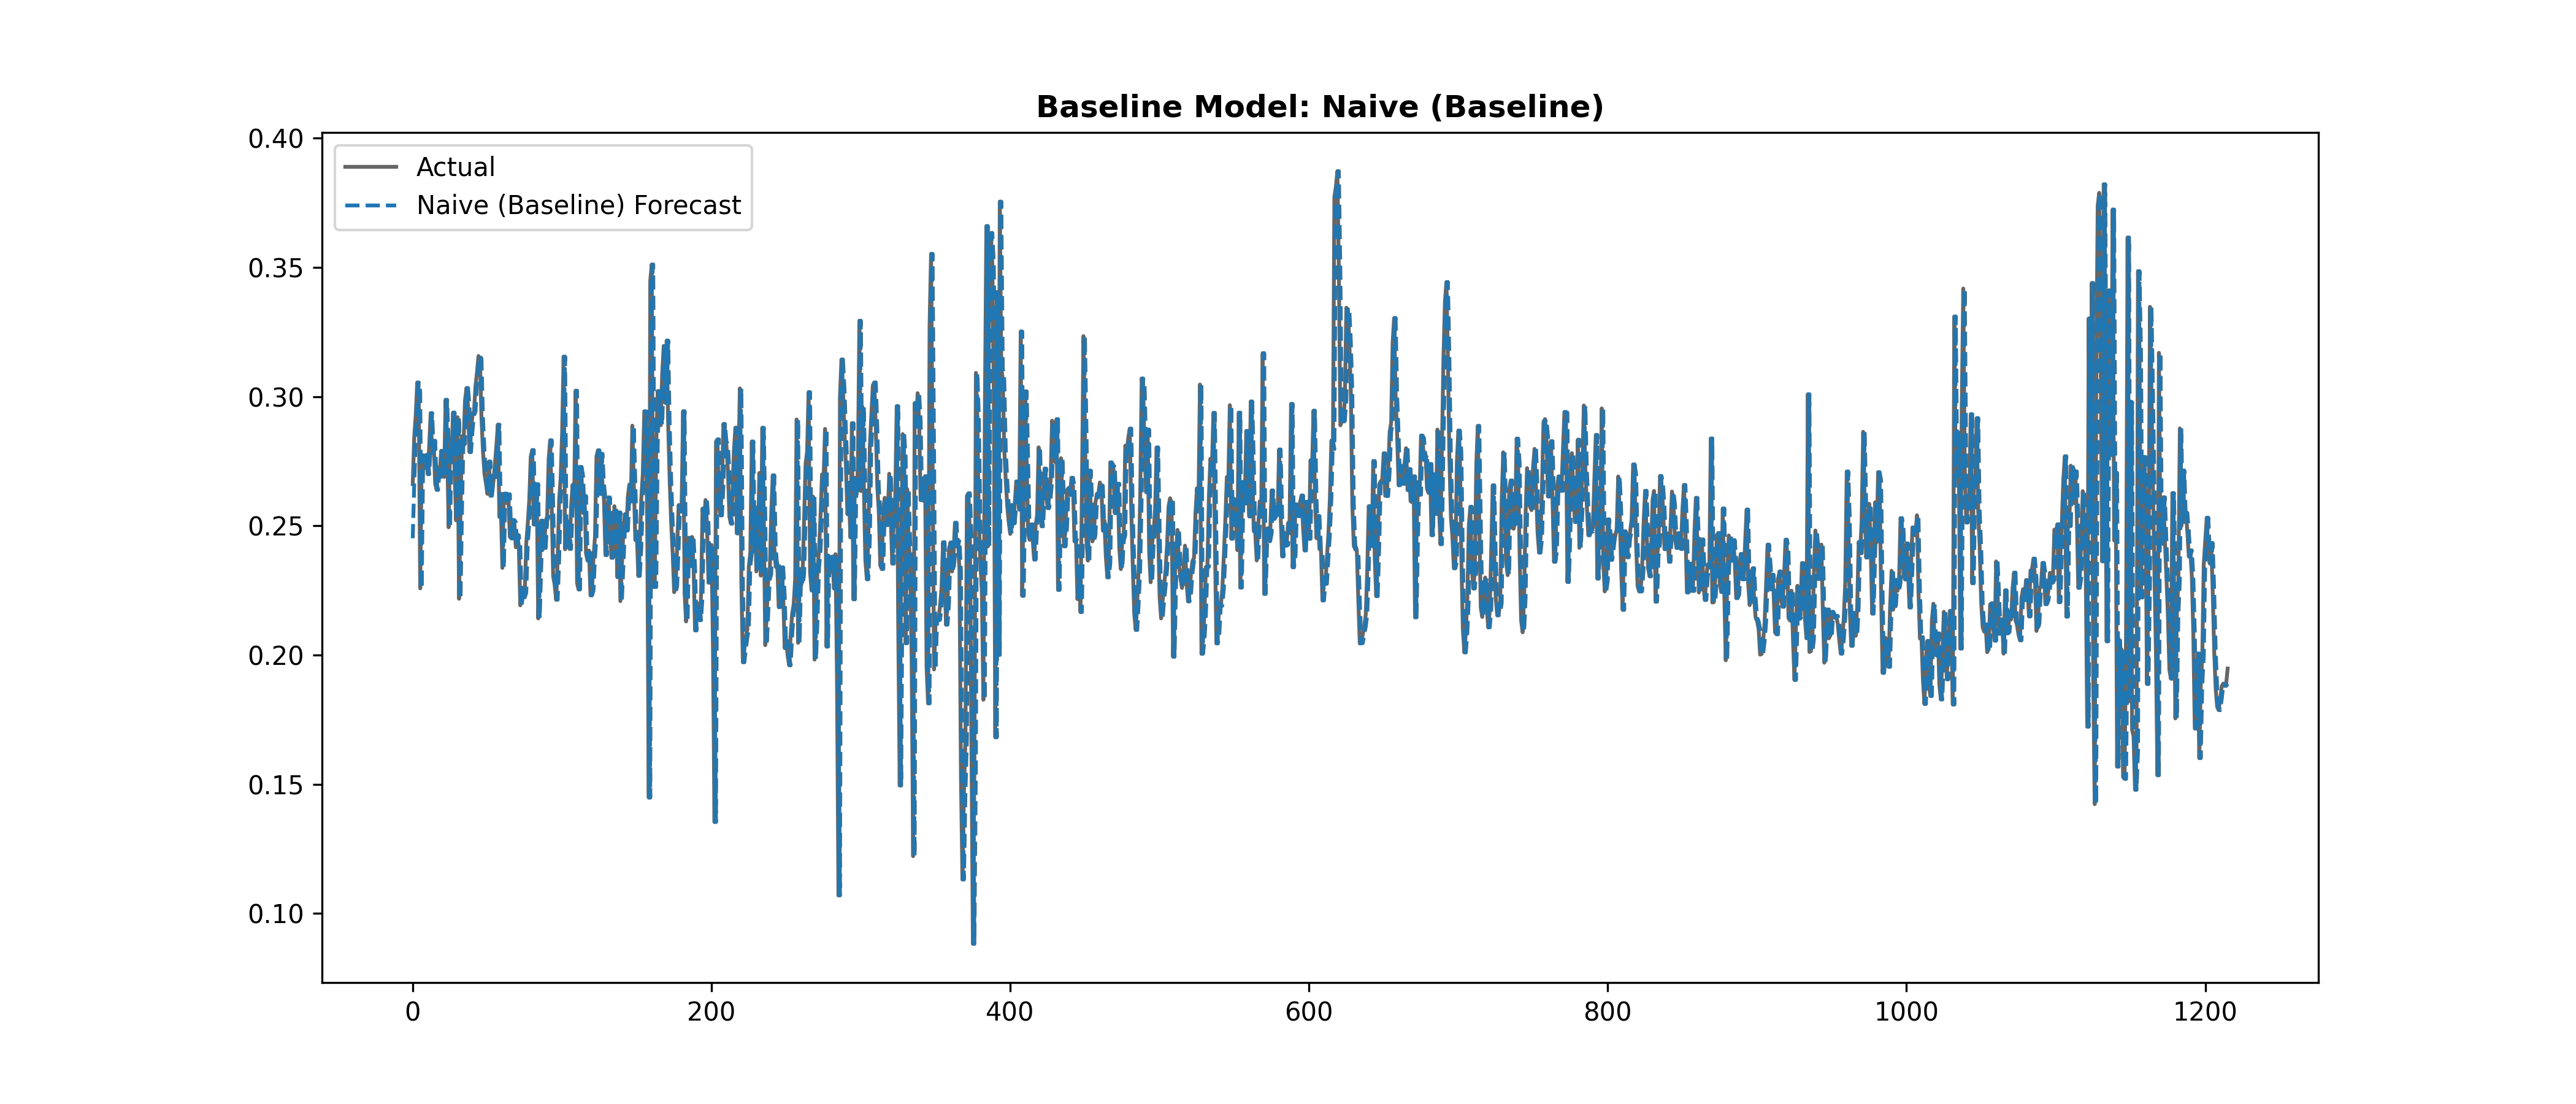
\includegraphics[width=\textwidth]{Forecasting_Graphs/00_Naive_(Baseline).png} \end{column}
        \begin{column}{0.33\textwidth} \metricwidget{Naive}{0.0211}{0.0345}{8.68}{0.0673} \end{column}
    \end{columns}
\end{frame}

\begin{frame}{Model 2: SMA-10}
    \textbf{\textcolor{VibrantAmber}{Theory:}} smoothing sensor jitter via 10s moving mean.
    \begin{columns}
        \begin{column}{0.65\textwidth} 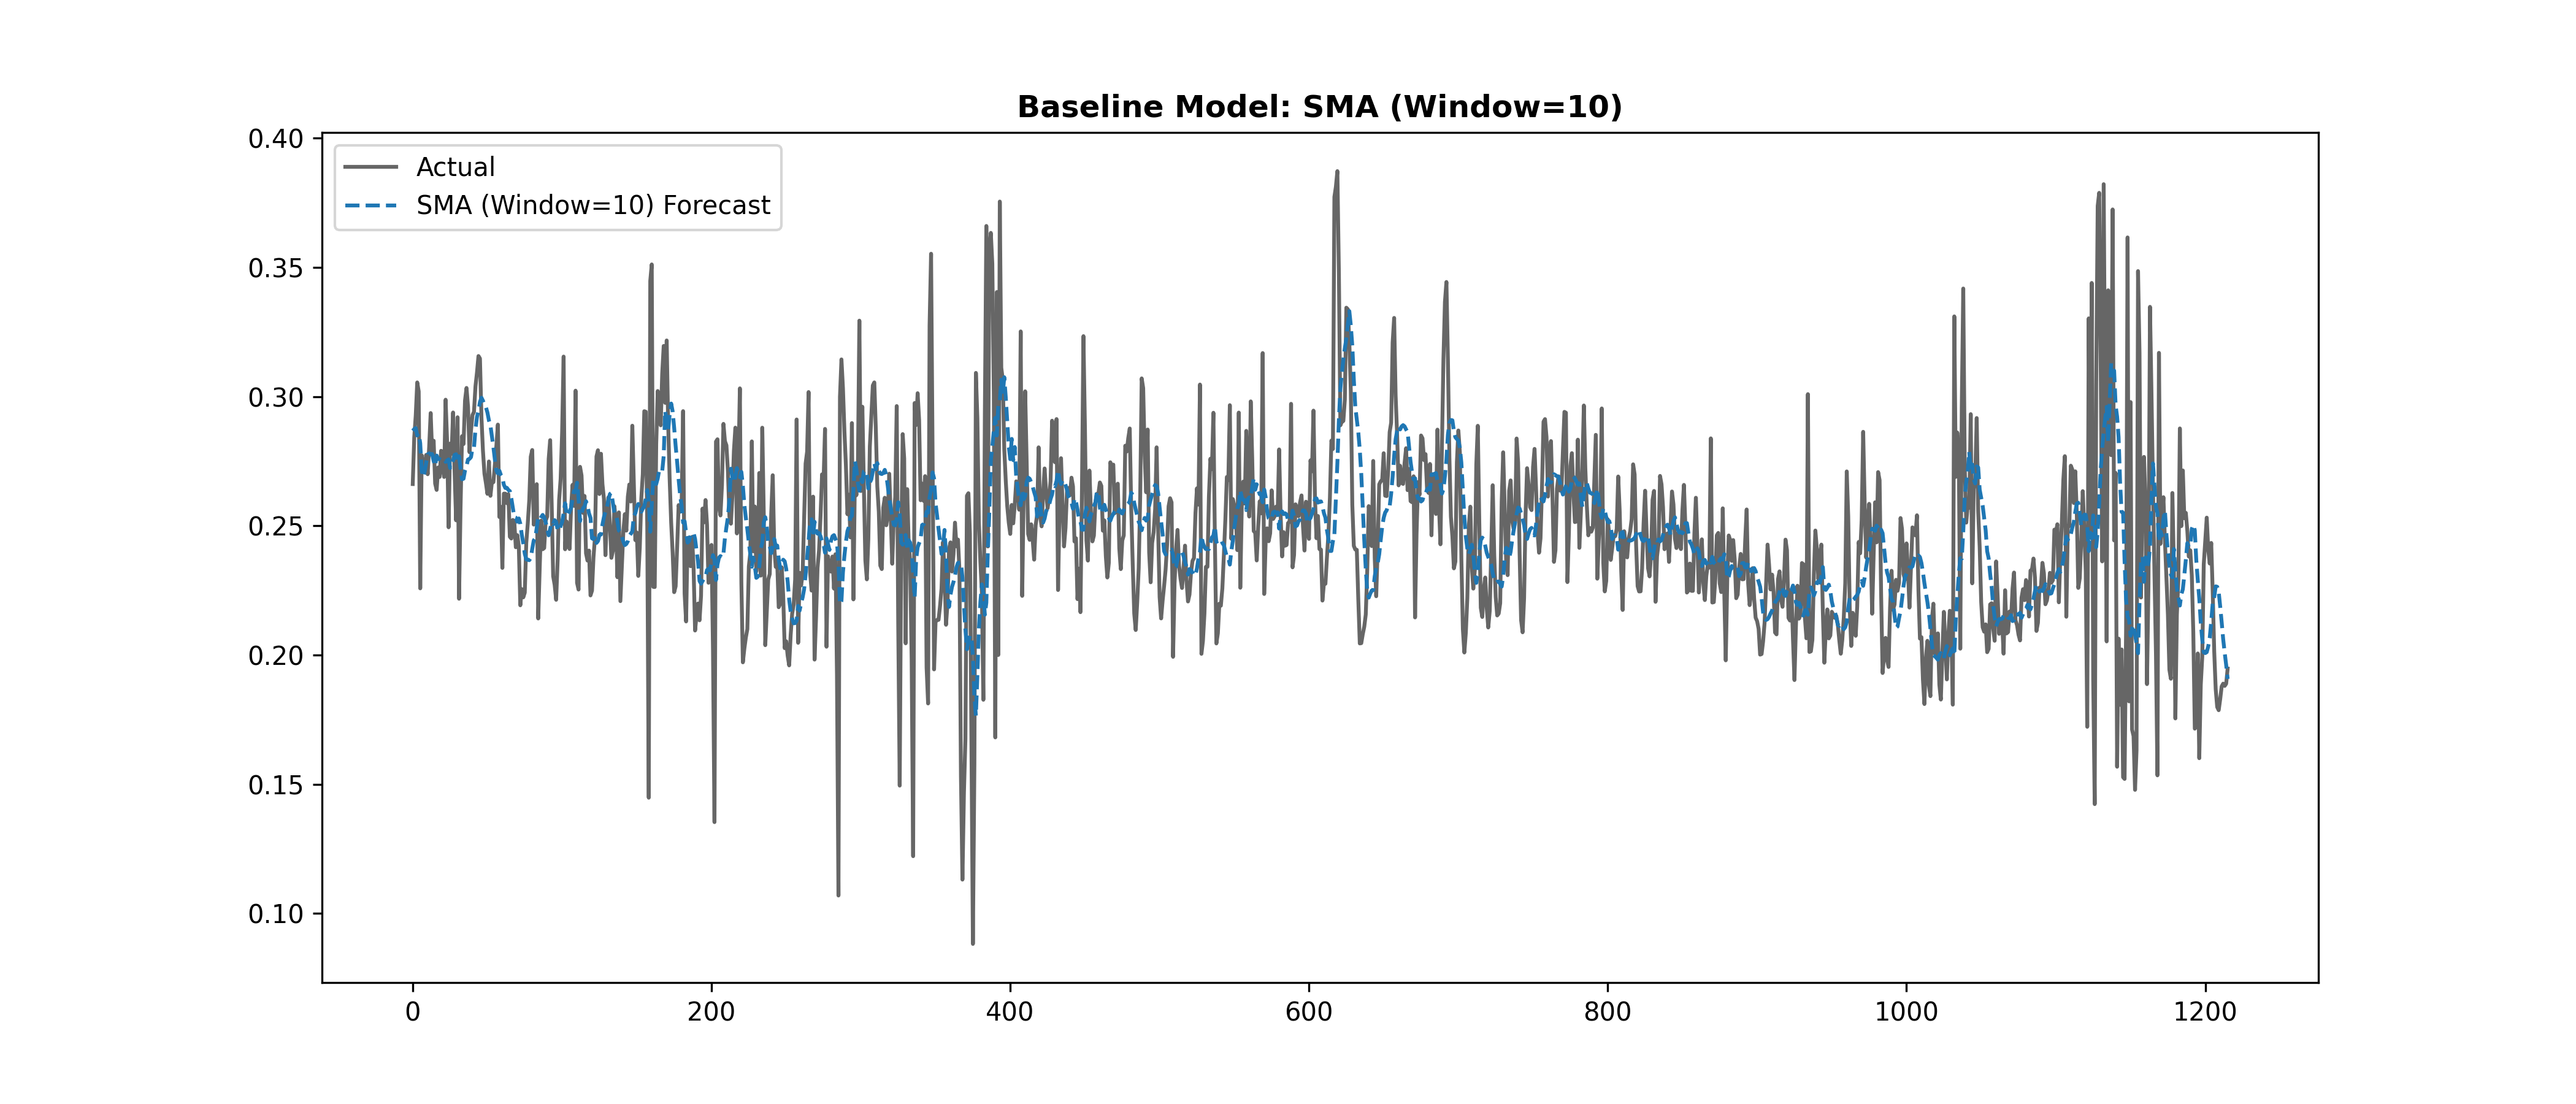
\includegraphics[width=\textwidth]{Forecasting_Graphs/00_SMA_(Window=10).png} \end{column}
        \begin{column}{0.33\textwidth} \metricwidget{SMA-10}{0.0229}{0.0326}{9.62}{0.1716} \end{column}
    \end{columns}
\end{frame}

\begin{frame}{Model 3: AR(2)}
    \textbf{\textcolor{VibrantAmber}{Theory:}} $y_t = c + \phi_1 y_{t-1} + \phi_2 y_{t-2} + \epsilon_t$
    \begin{columns}
        \begin{column}{0.65\textwidth} 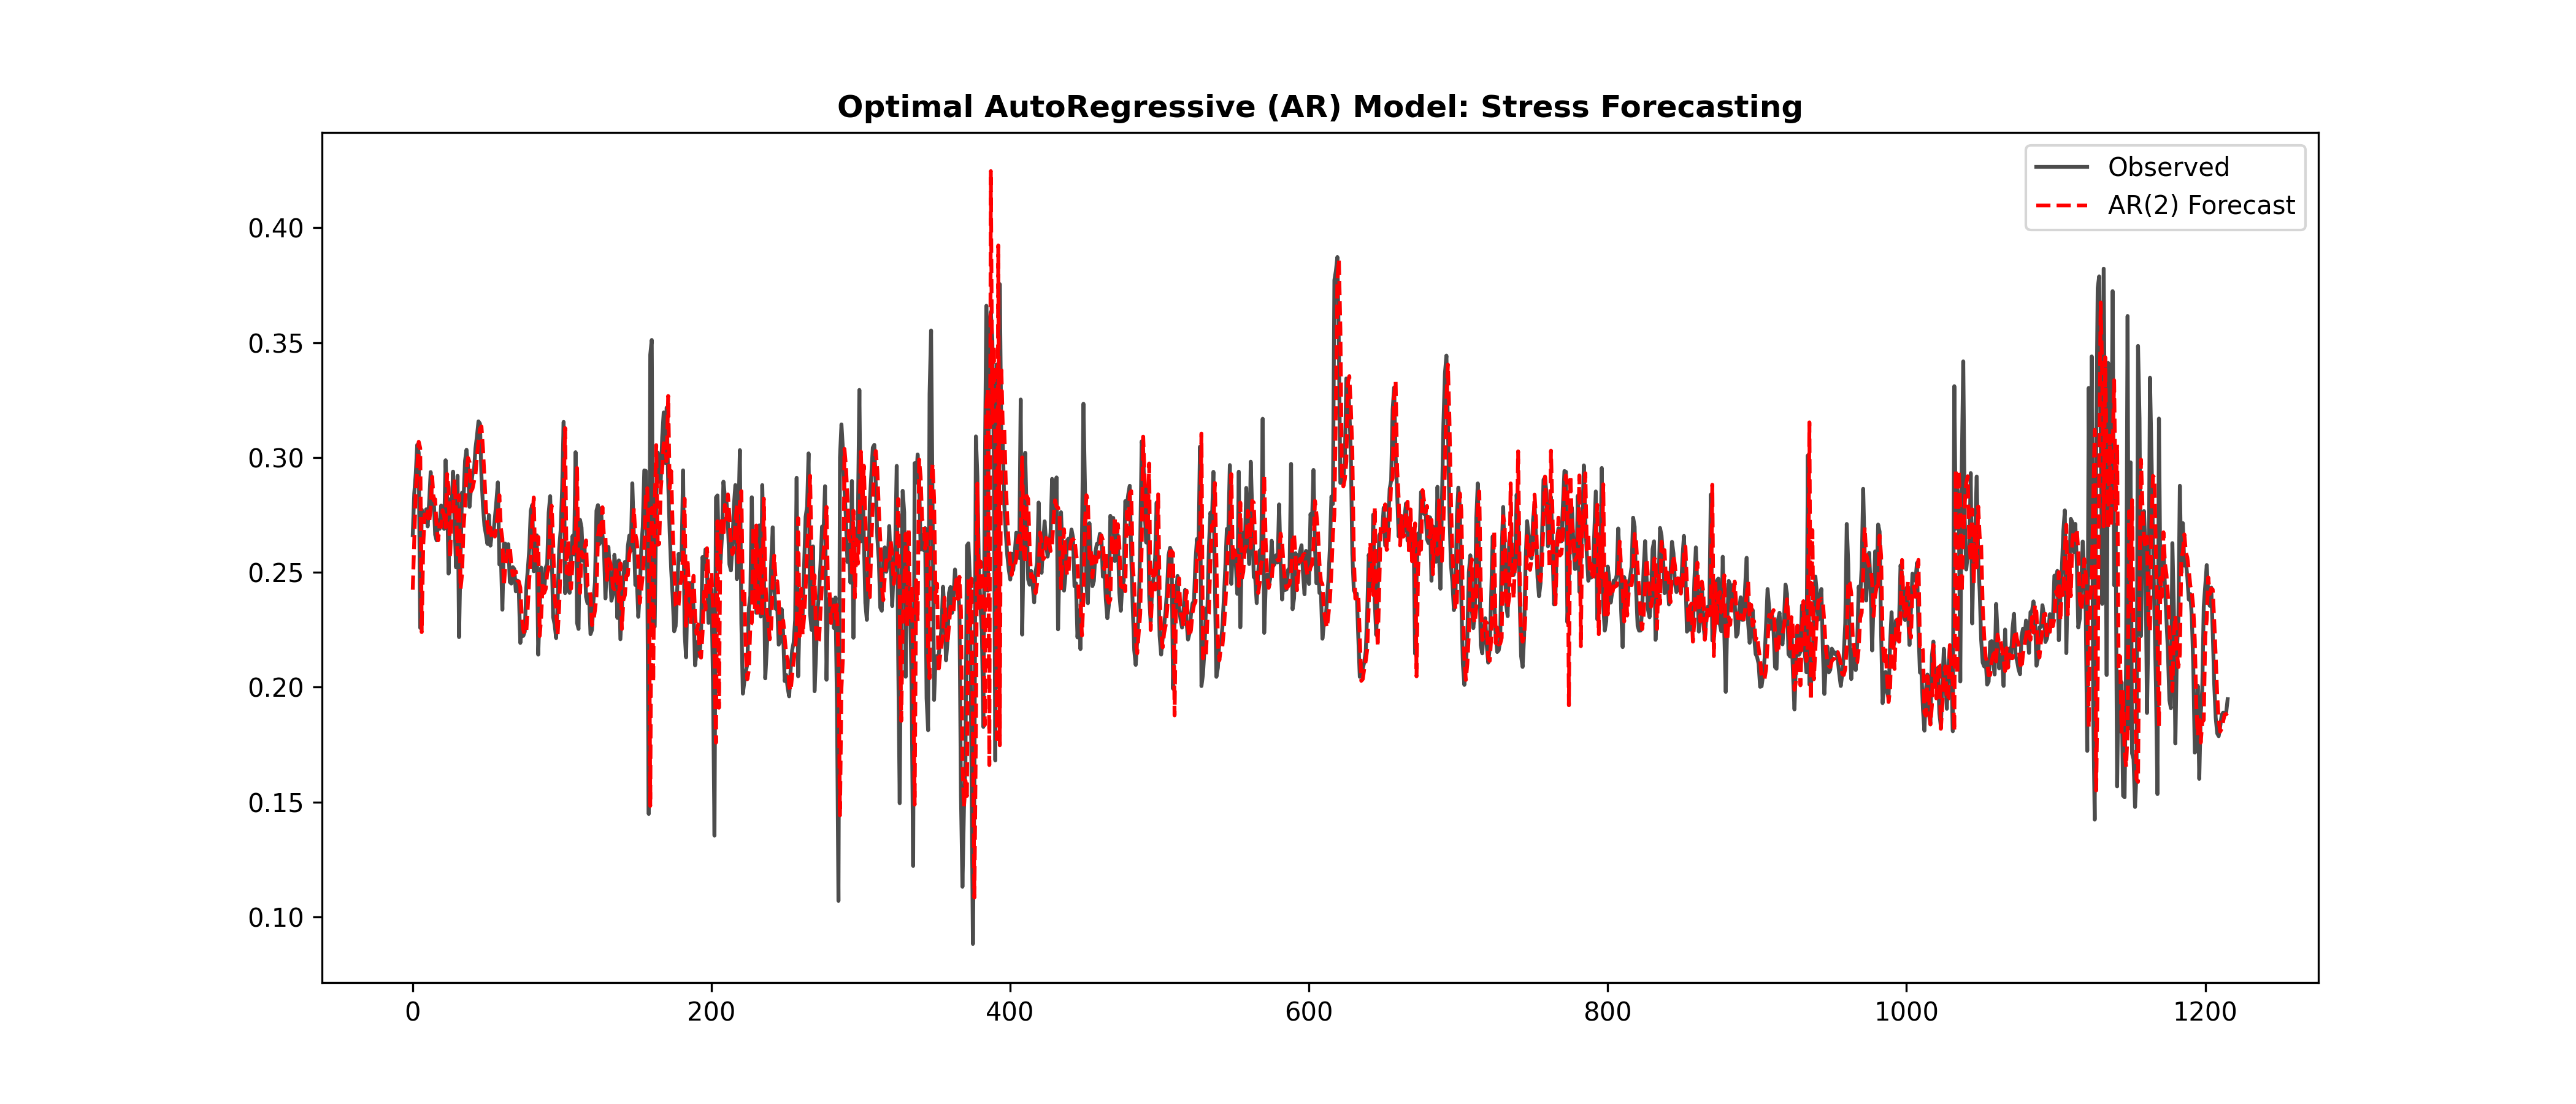
\includegraphics[width=\textwidth]{Forecasting_Graphs/03_AR_Optimized.png} \end{column}
        \begin{column}{0.33\textwidth} \metricwidget{AR(2)}{0.0210}{0.0342}{8.66}{0.0840} \end{column}
    \end{columns}
\end{frame}

\begin{frame}{Model 4: MA(3)}
    \textbf{\textcolor{VibrantAmber}{Theory:}} error-correction based on 3 shock terms.
    \begin{columns}
        \begin{column}{0.65\textwidth} 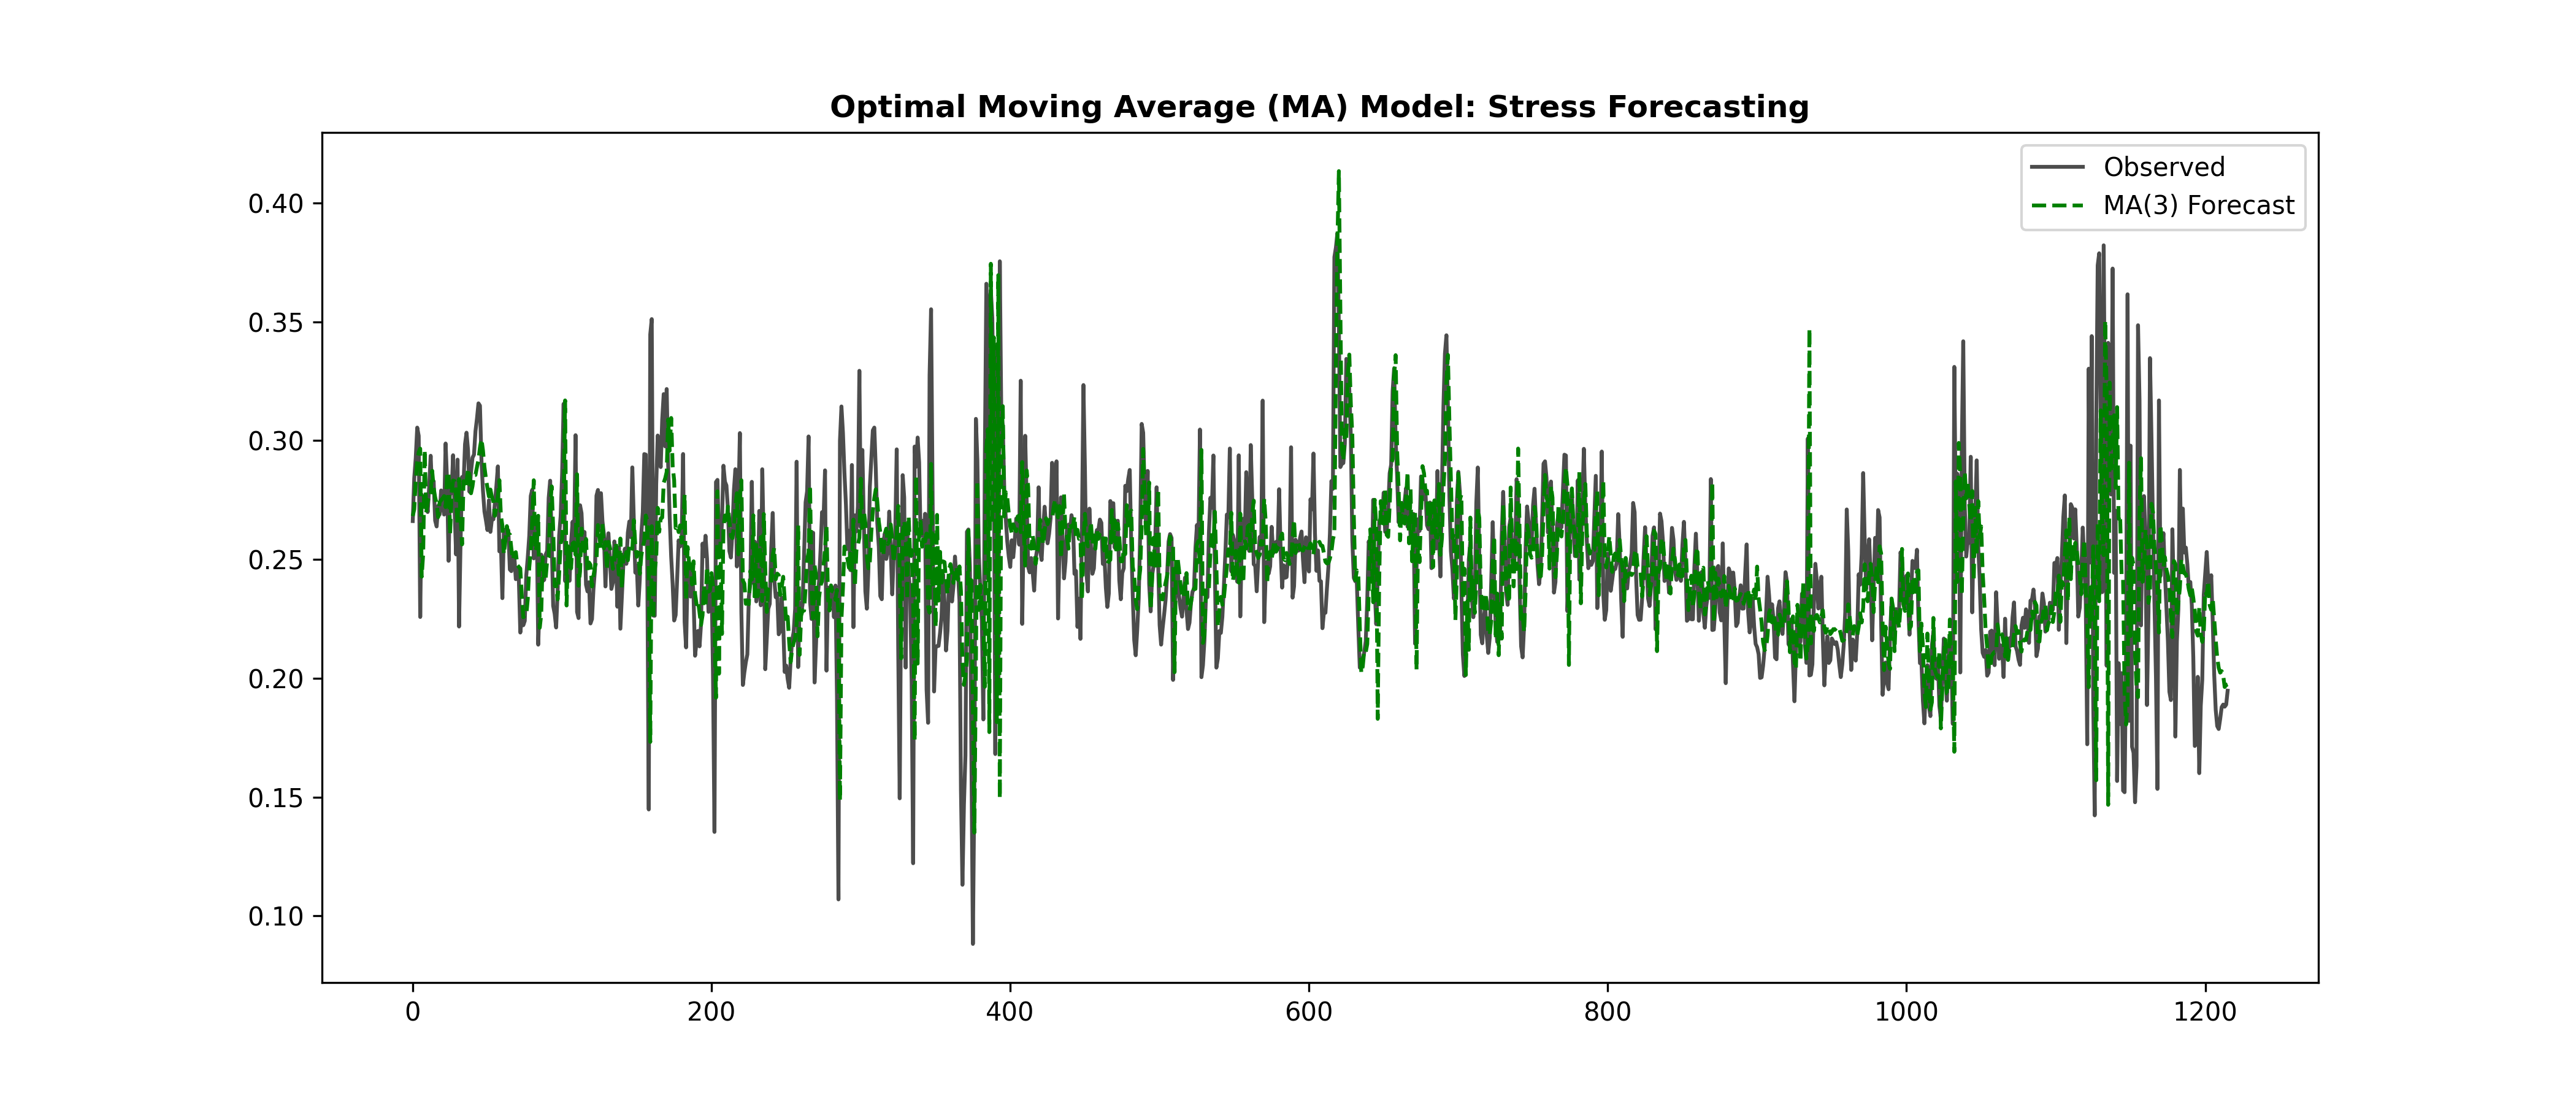
\includegraphics[width=\textwidth]{Forecasting_Graphs/04_MA_Optimized.png} \end{column}
        \begin{column}{0.33\textwidth} \metricwidget{MA(3)}{0.0209}{0.0335}{8.72}{0.1236} \end{column}
    \end{columns}
\end{frame}

\begin{frame}{Model 5: ARMA(2,3)}
    \textbf{\textcolor{VibrantAmber}{Theory:}} AIC-optimized linear hybrid.
    \begin{columns}
        \begin{column}{0.65\textwidth} 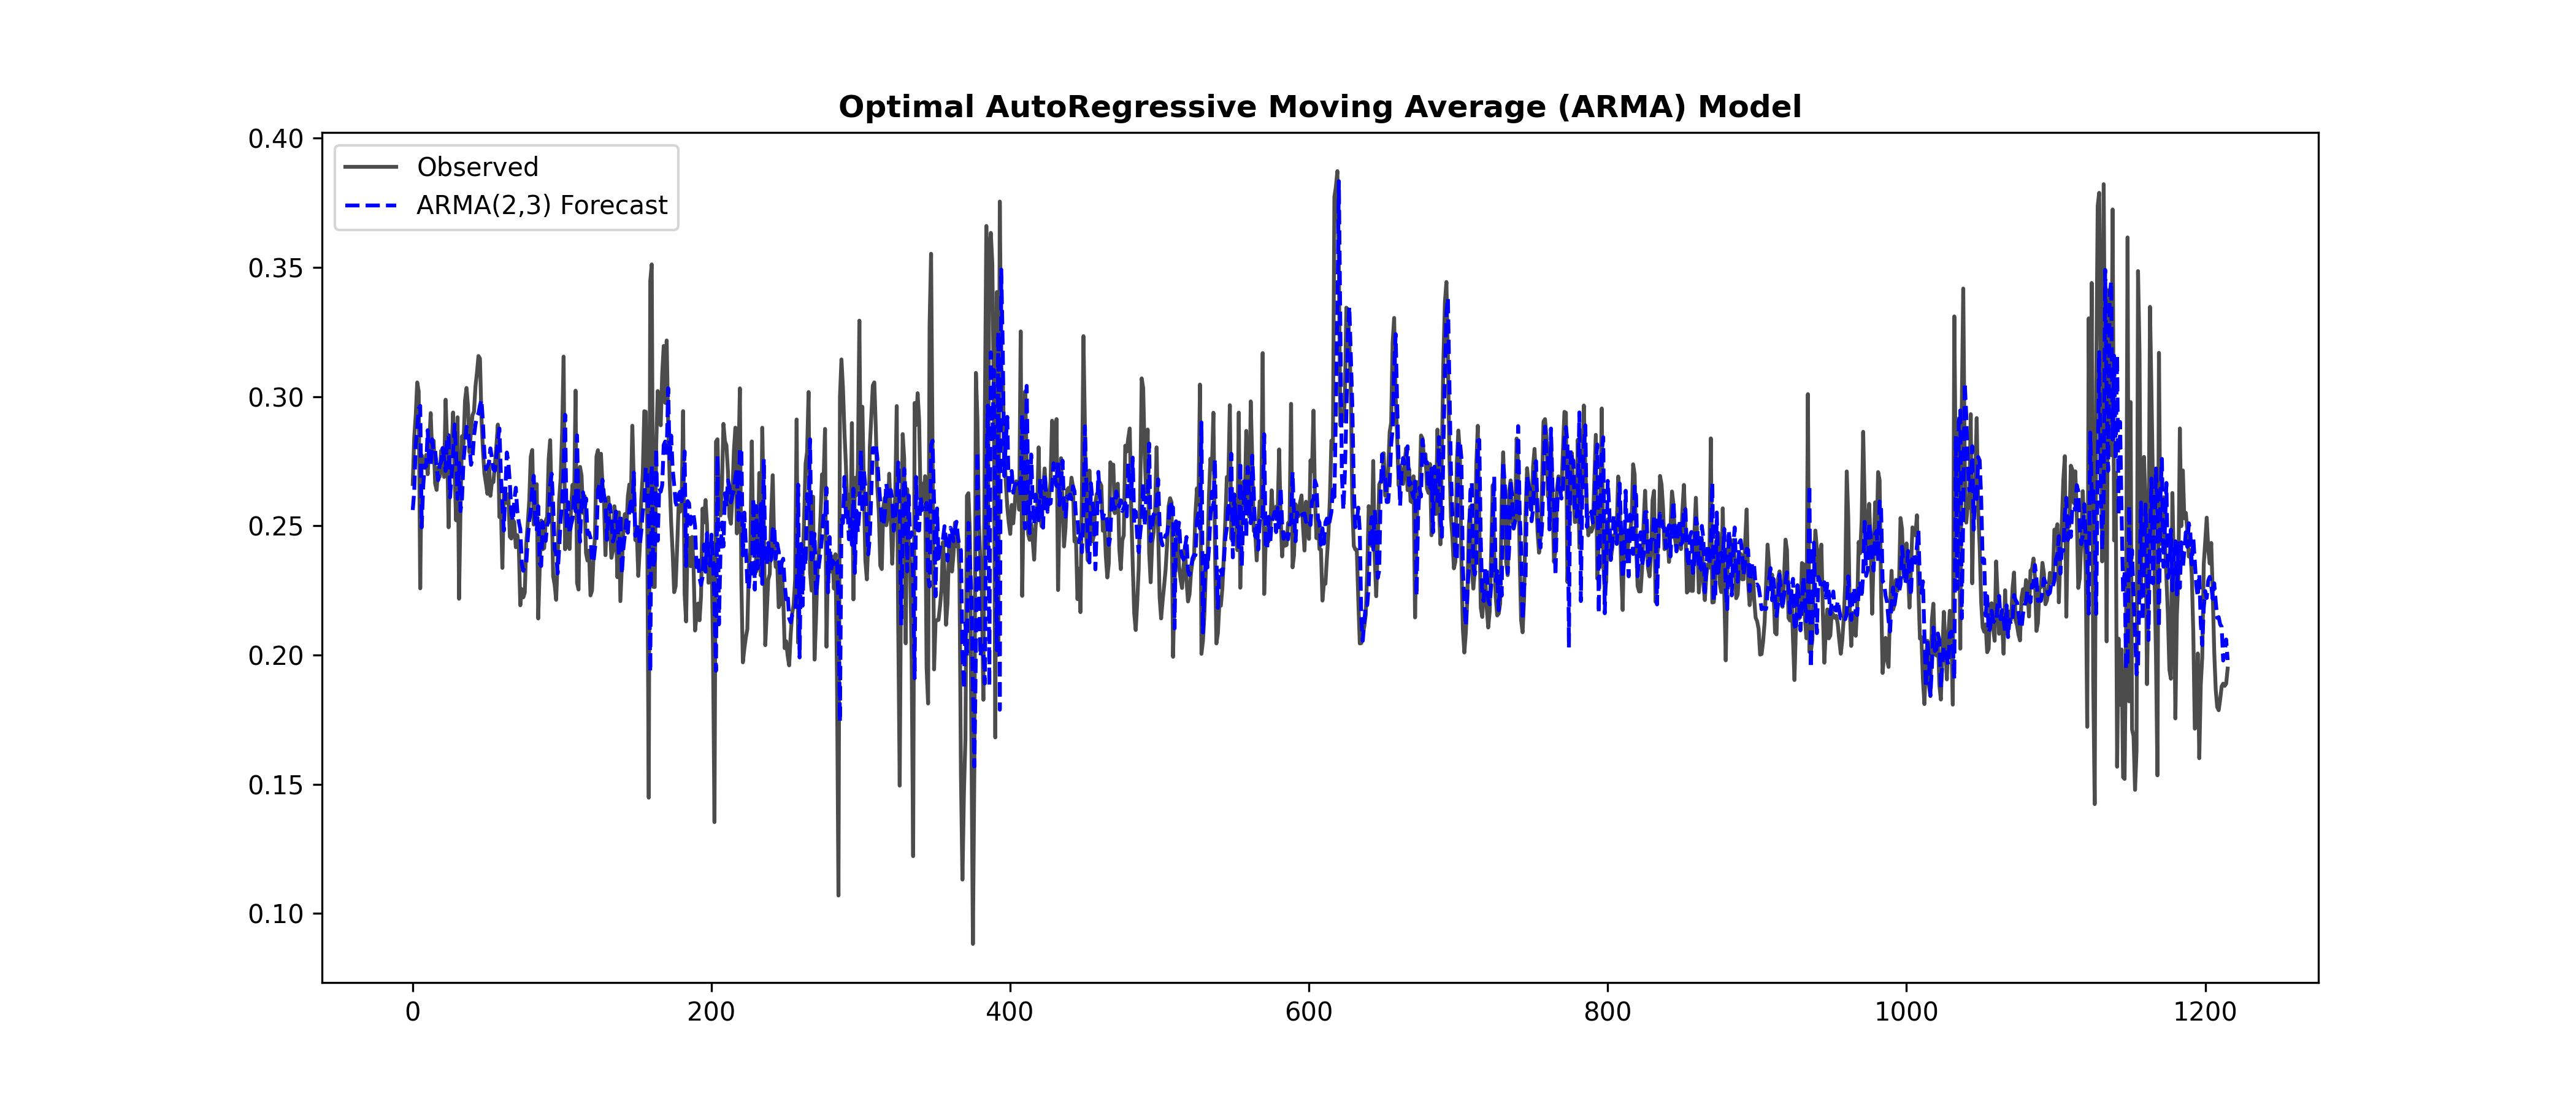
\includegraphics[width=\textwidth]{Forecasting_Graphs/05_ARMA_Optimized.png} \end{column}
        \begin{column}{0.33\textwidth} \metricwidget{ARMA(2,3)}{0.0206}{0.0316}{8.60}{0.2204} \end{column}
    \end{columns}
\end{frame}

\begin{frame}{Model 6: SARIMA}
    \textbf{\textcolor{VibrantAmber}{Theory:}} 7s seasonal periodicity integration.
    \begin{columns}
        \begin{column}{0.65\textwidth} 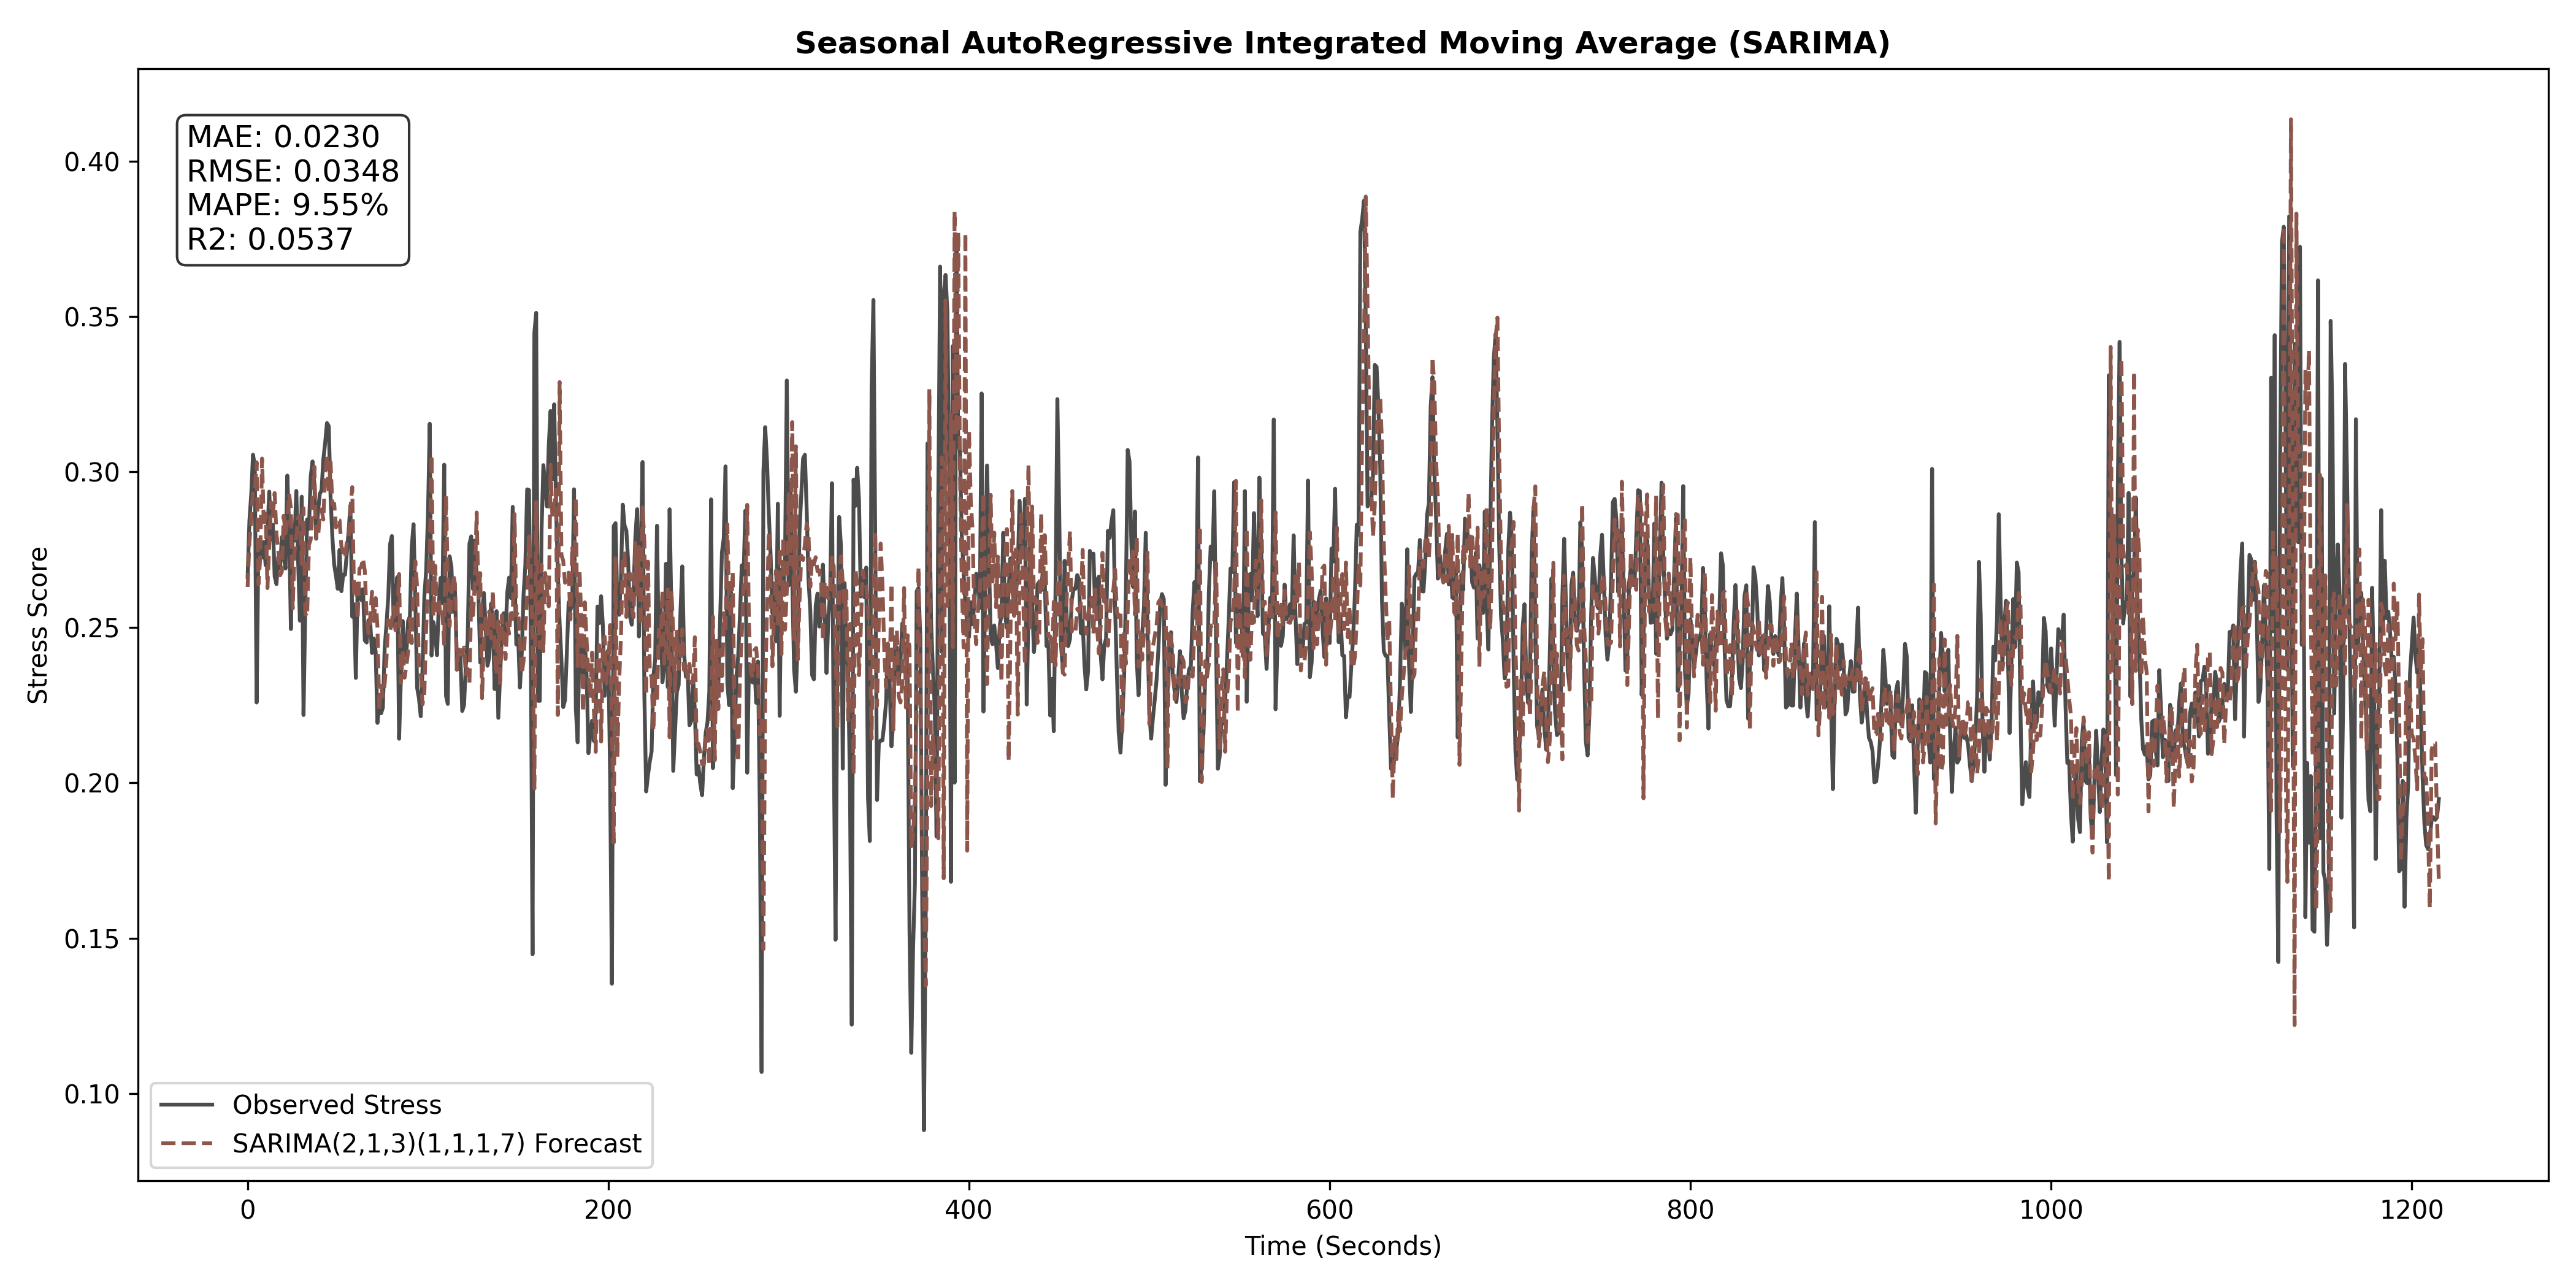
\includegraphics[width=\textwidth]{Forecasting_Graphs/06_SARIMA_Optimized.png} \end{column}
        \begin{column}{0.33\textwidth} \metricwidget{SARIMA}{0.0230}{0.0348}{9.55}{0.0537} \end{column}
    \end{columns}
\end{frame}

\begin{frame}{Model 7: SARIMAX}
    \textbf{\textcolor{VibrantAmber}{Theory:}} SARIMA + Lagged Physiological Predictors.
    \begin{columns}
        \begin{column}{0.65\textwidth} 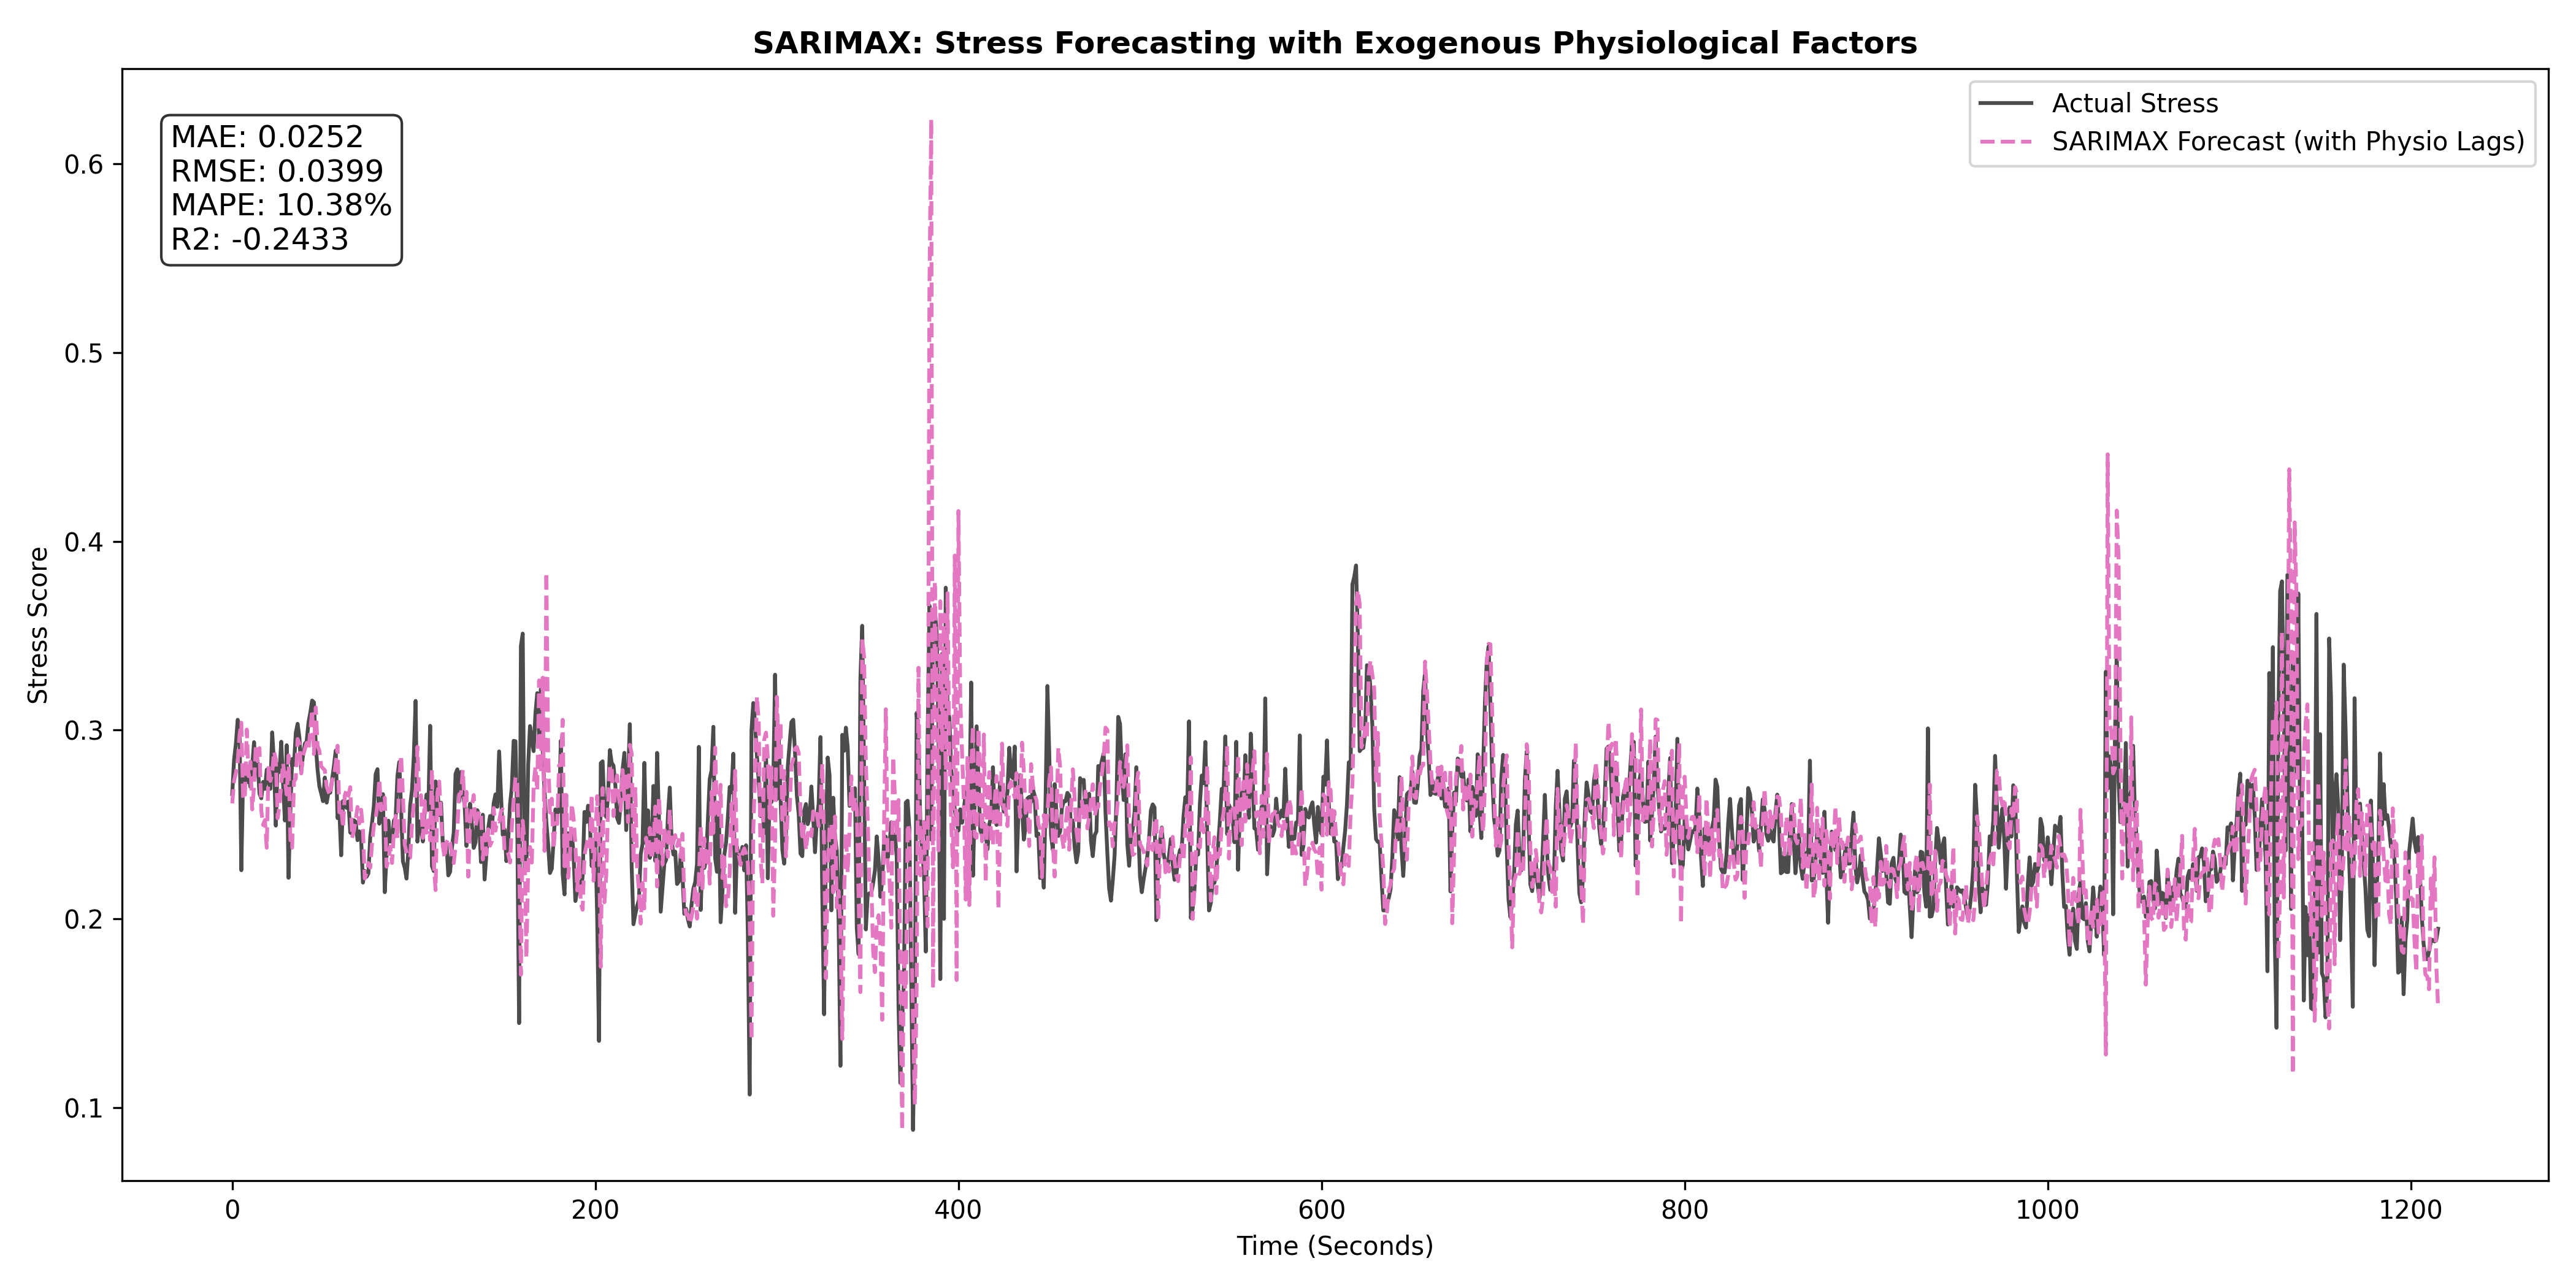
\includegraphics[width=\textwidth]{Forecasting_Graphs/07_SARIMAX_Optimized.png} \end{column}
        \begin{column}{0.33\textwidth} \metricwidget{SARIMAX}{0.0252}{0.0399}{10.38}{-0.2433} \end{column}
    \end{columns}
\end{frame}

\begin{frame}{Model 8: Random Forest}
    \begin{columns}
        \begin{column}{0.65\textwidth} 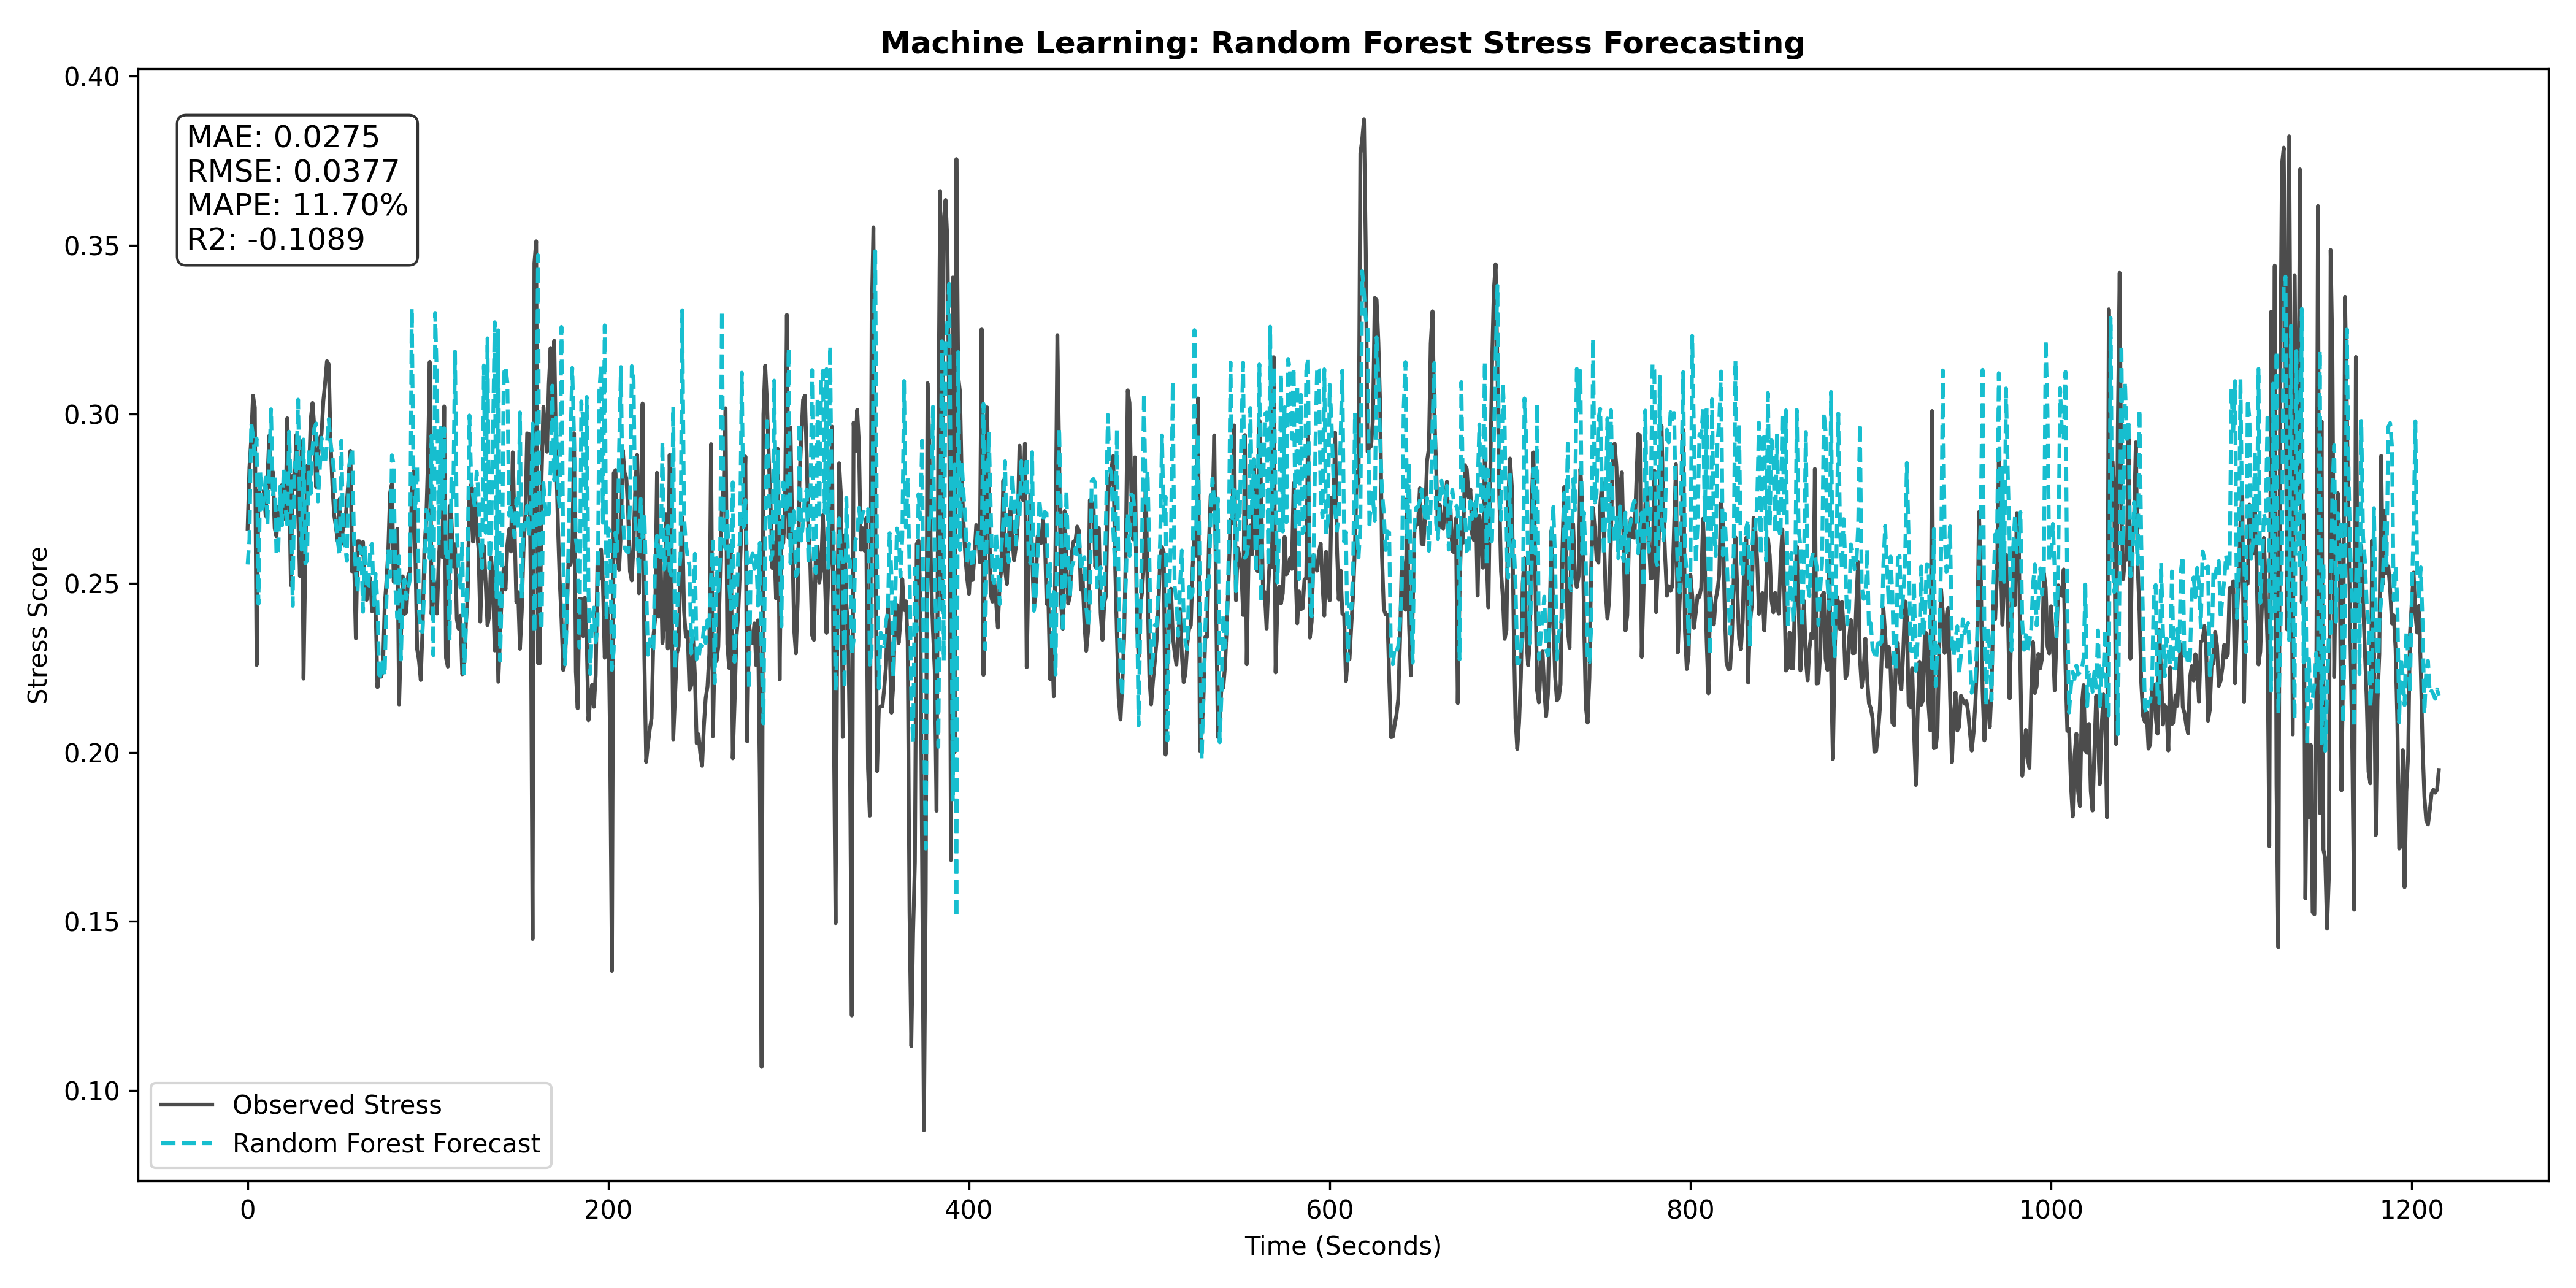
\includegraphics[width=\textwidth]{Forecasting_Graphs/08_Random_Forest_Forecast.png} \end{column}
        \begin{column}{0.33\textwidth} \metricwidget{RF}{0.0275}{0.0377}{11.70}{-0.1089} \end{column}
    \end{columns}
\end{frame}

\begin{frame}{Model 9: XGBoost}
    \begin{columns}
        \begin{column}{0.65\textwidth} 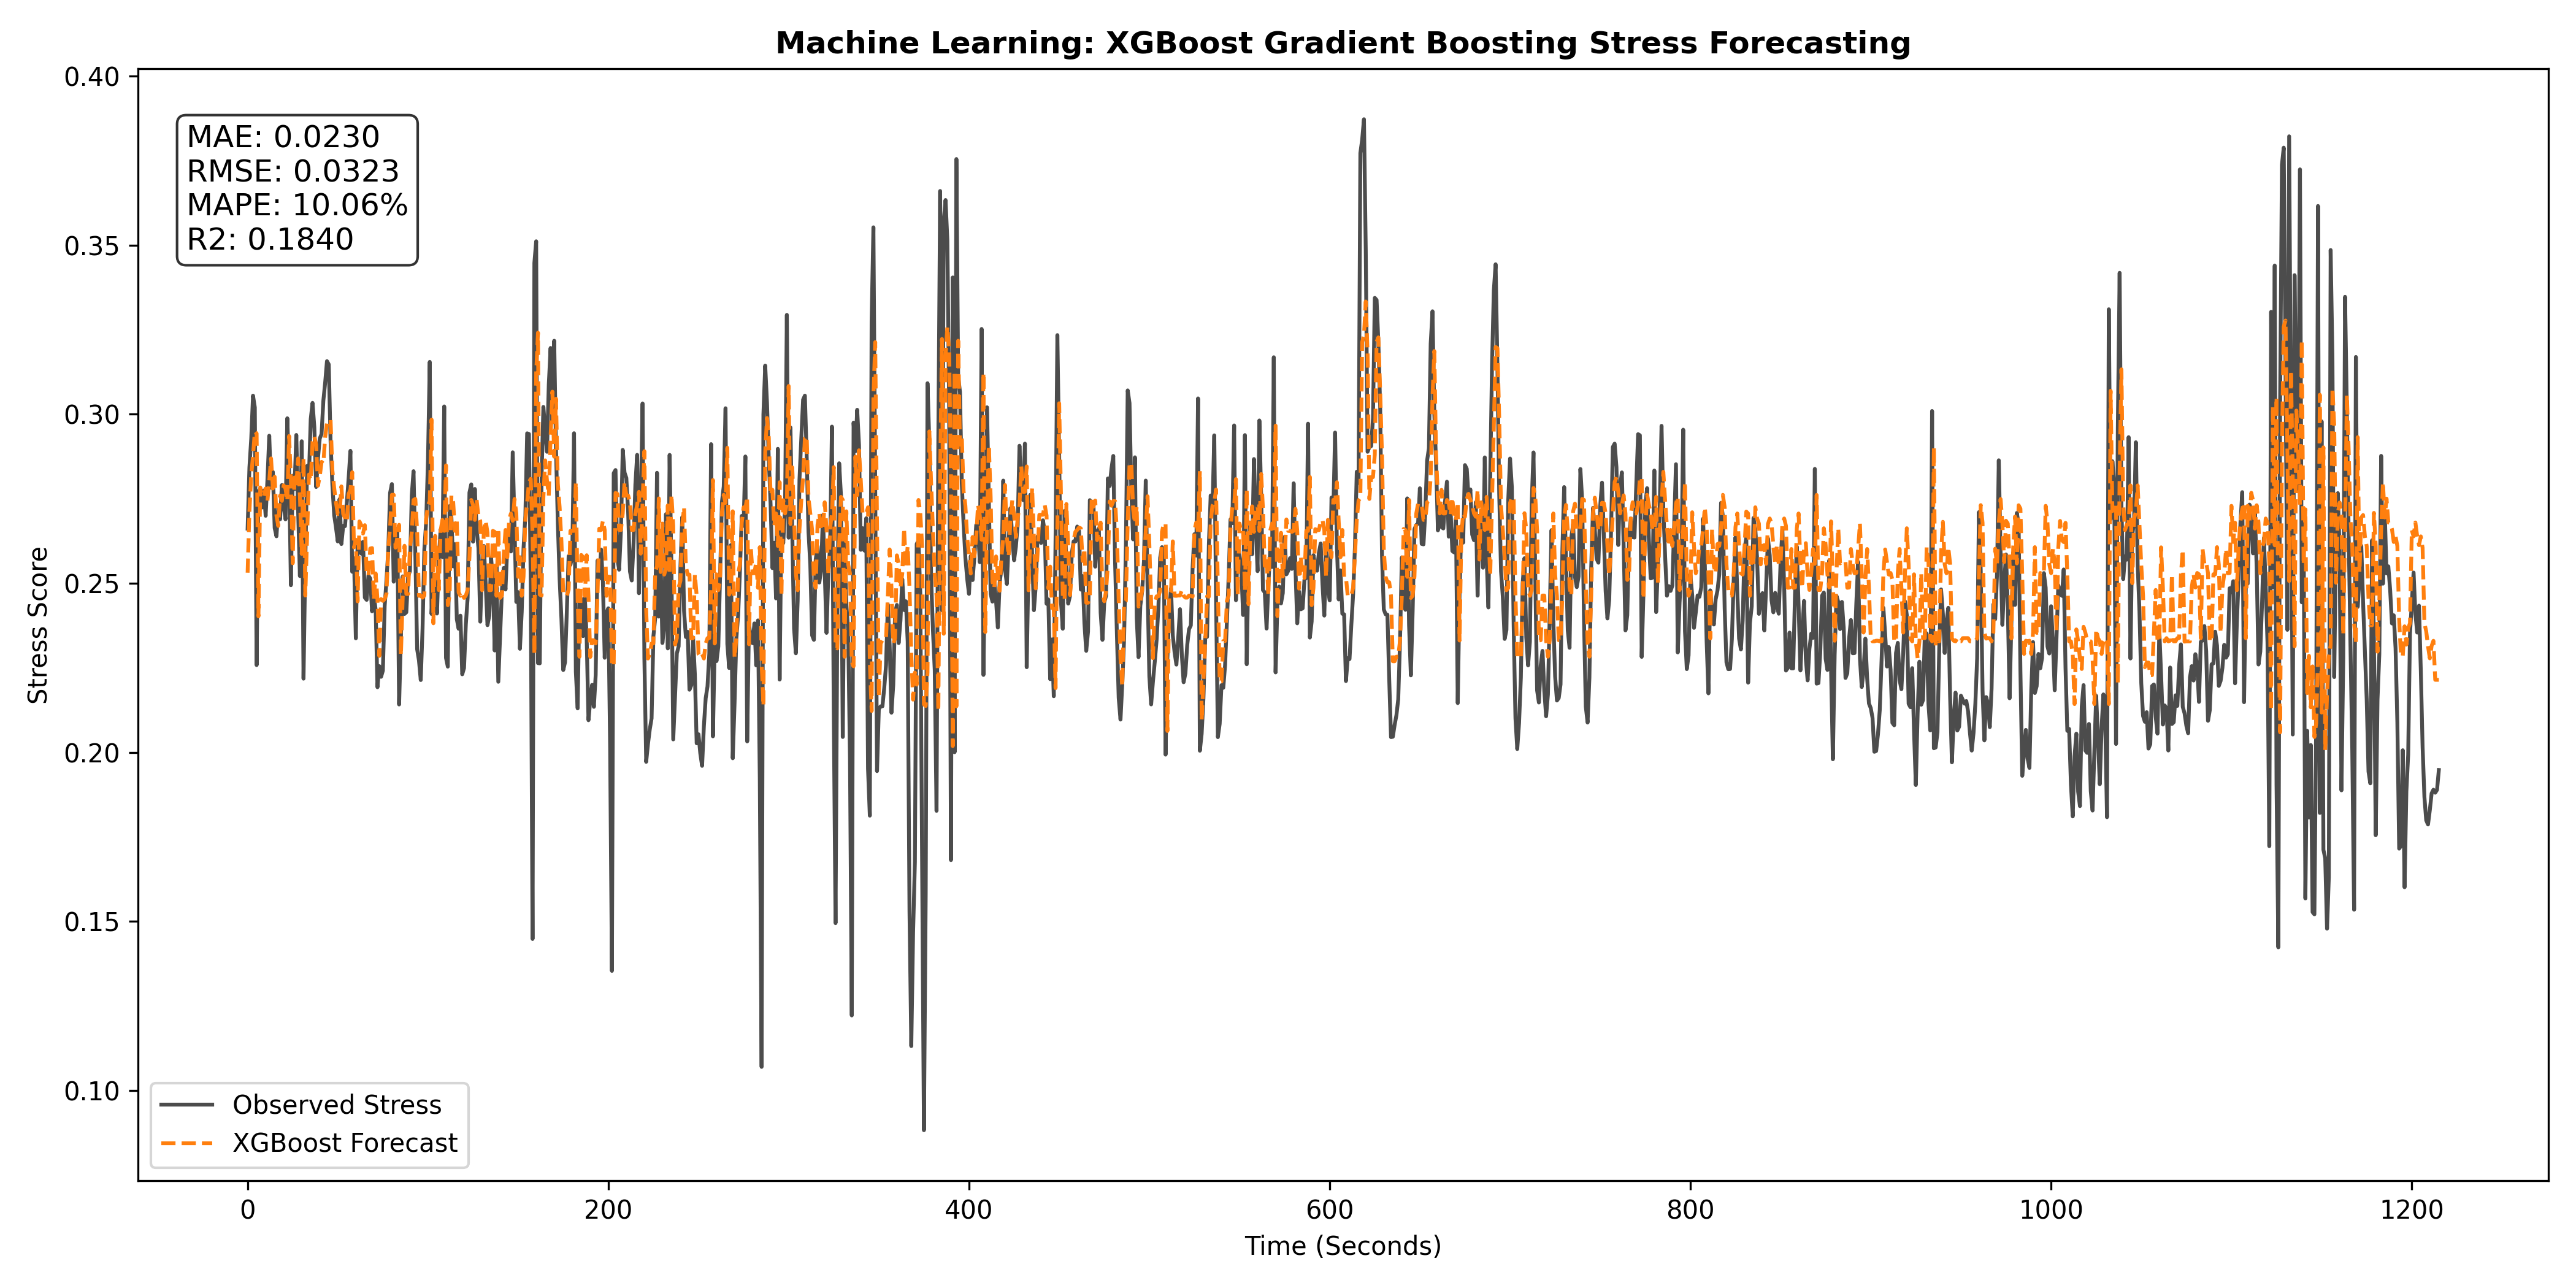
\includegraphics[width=\textwidth]{Forecasting_Graphs/09_XGBoost_Forecast.png} \end{column}
        \begin{column}{0.33\textwidth} \metricwidget{XGBoost}{0.0230}{0.0323}{10.06}{0.1840} \end{column}
    \end{columns}
\end{frame}

\begin{frame}{Model 10: LSTM}
    \begin{columns}
        \begin{column}{0.65\textwidth} 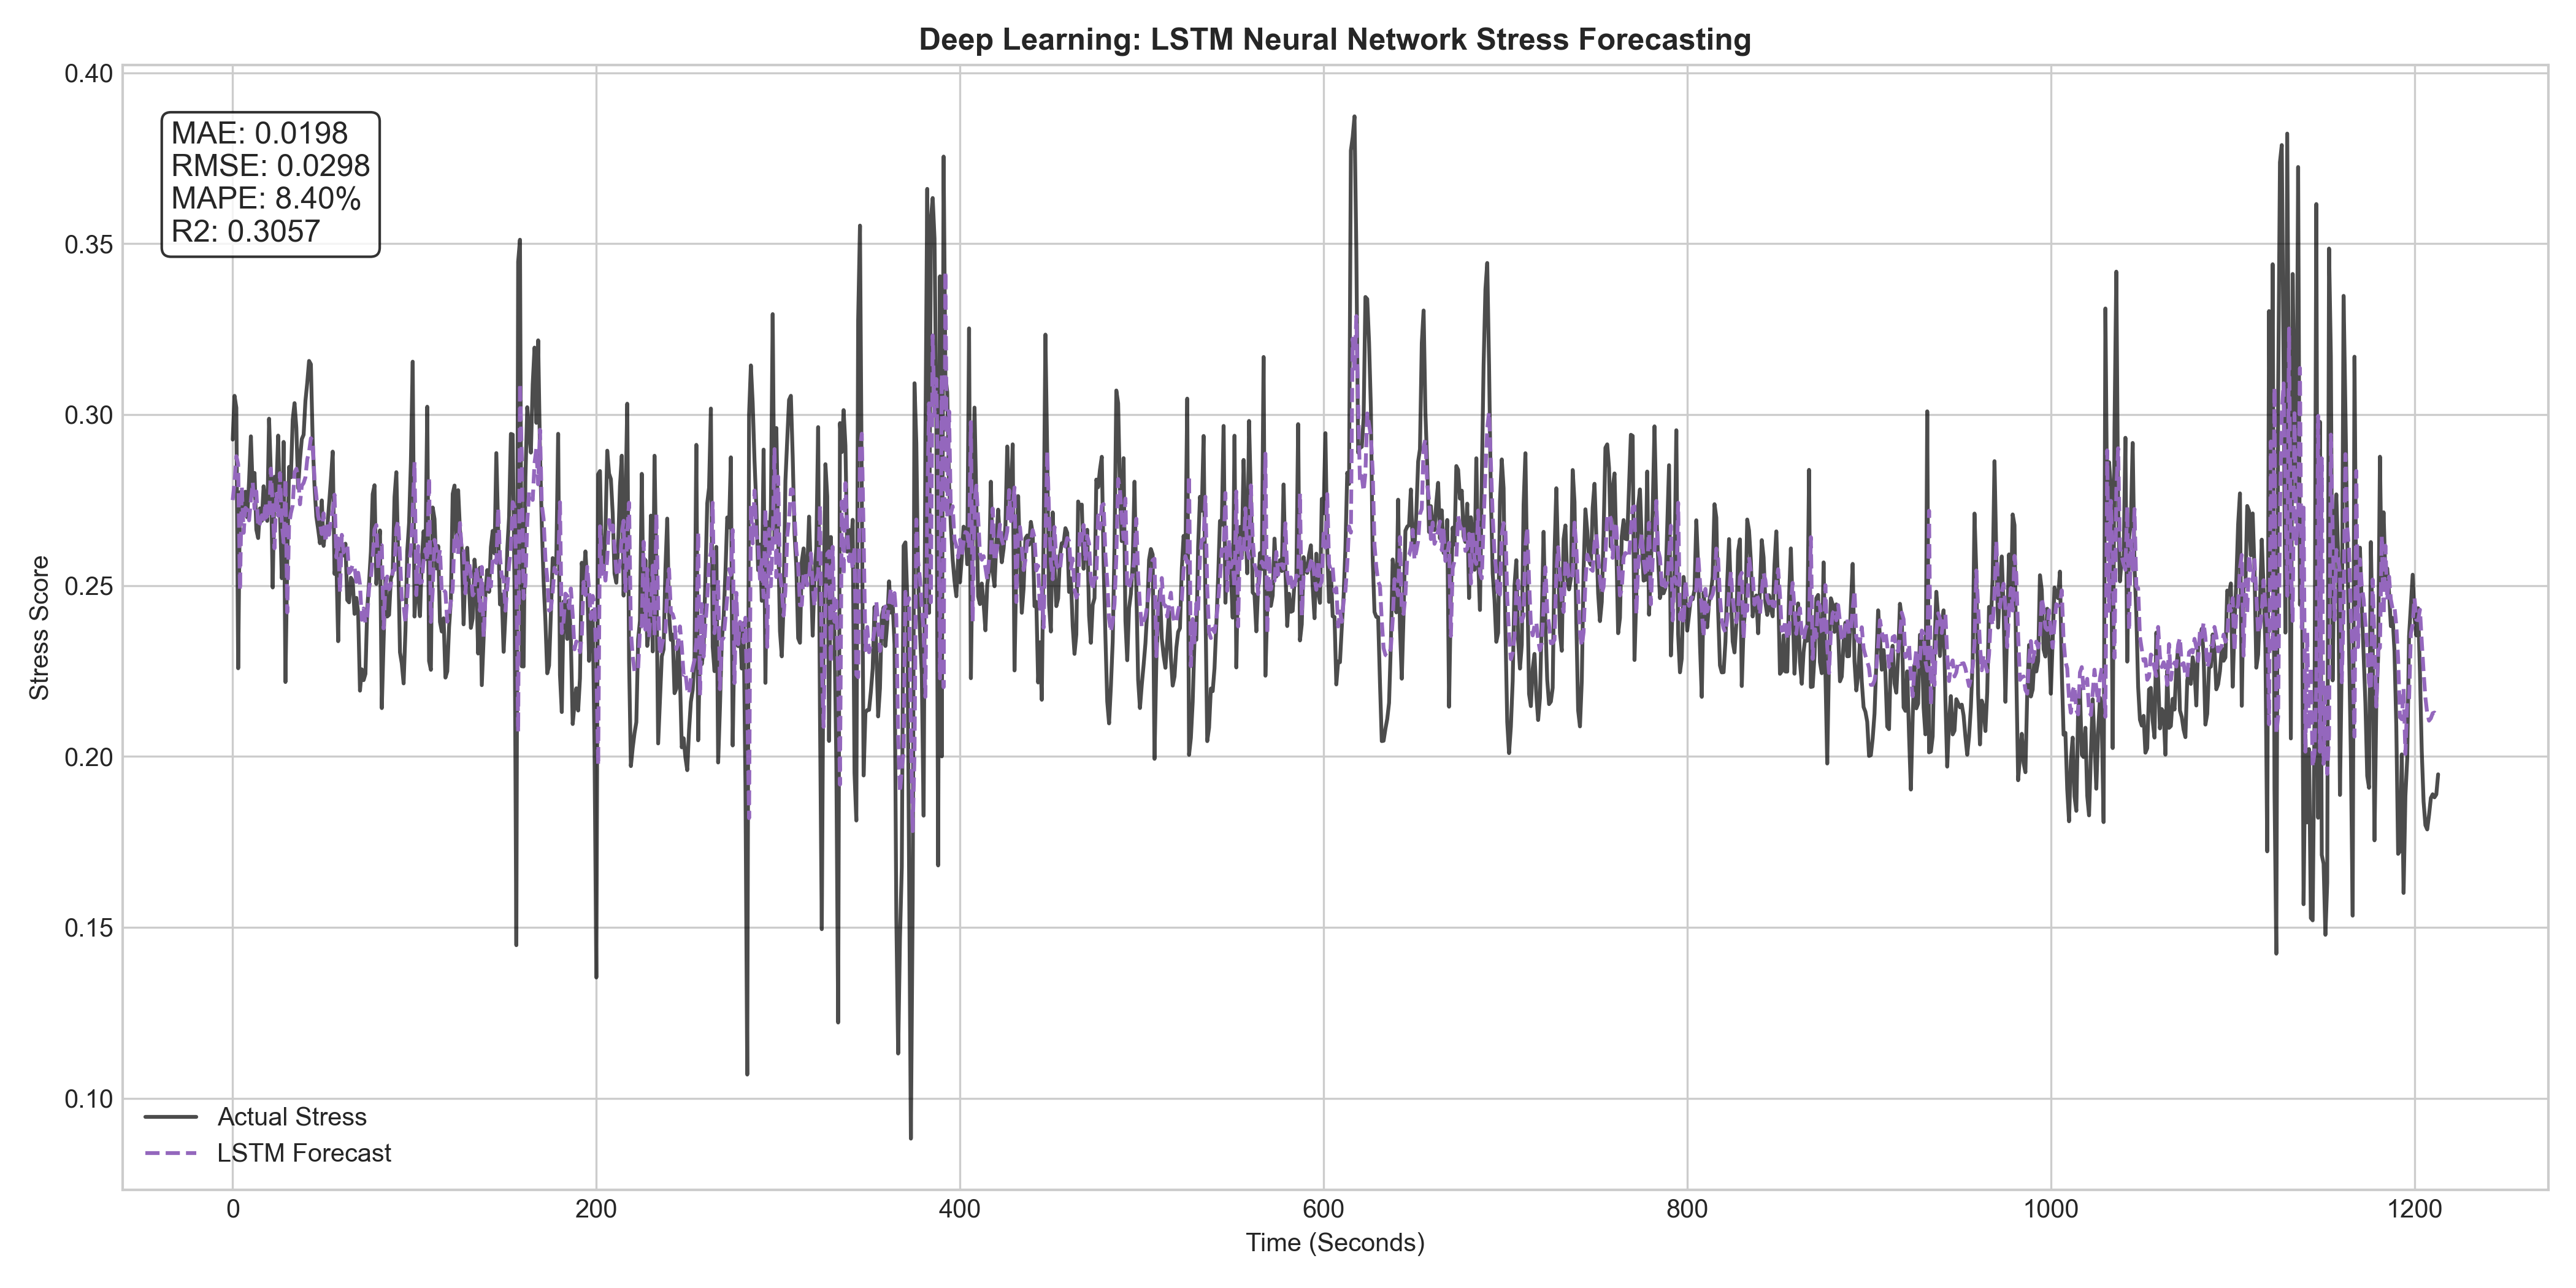
\includegraphics[width=\textwidth]{Forecasting_Graphs/10_LSTM_Forecast.png} \end{column}
        \begin{column}{0.33\textwidth} \metricwidget{LSTM}{0.0198}{0.0298}{8.40}{0.3057} \end{column}
    \end{columns}
\end{frame}

\begin{frame}{Model 11: SVR}
    \begin{columns}
        \begin{column}{0.65\textwidth} 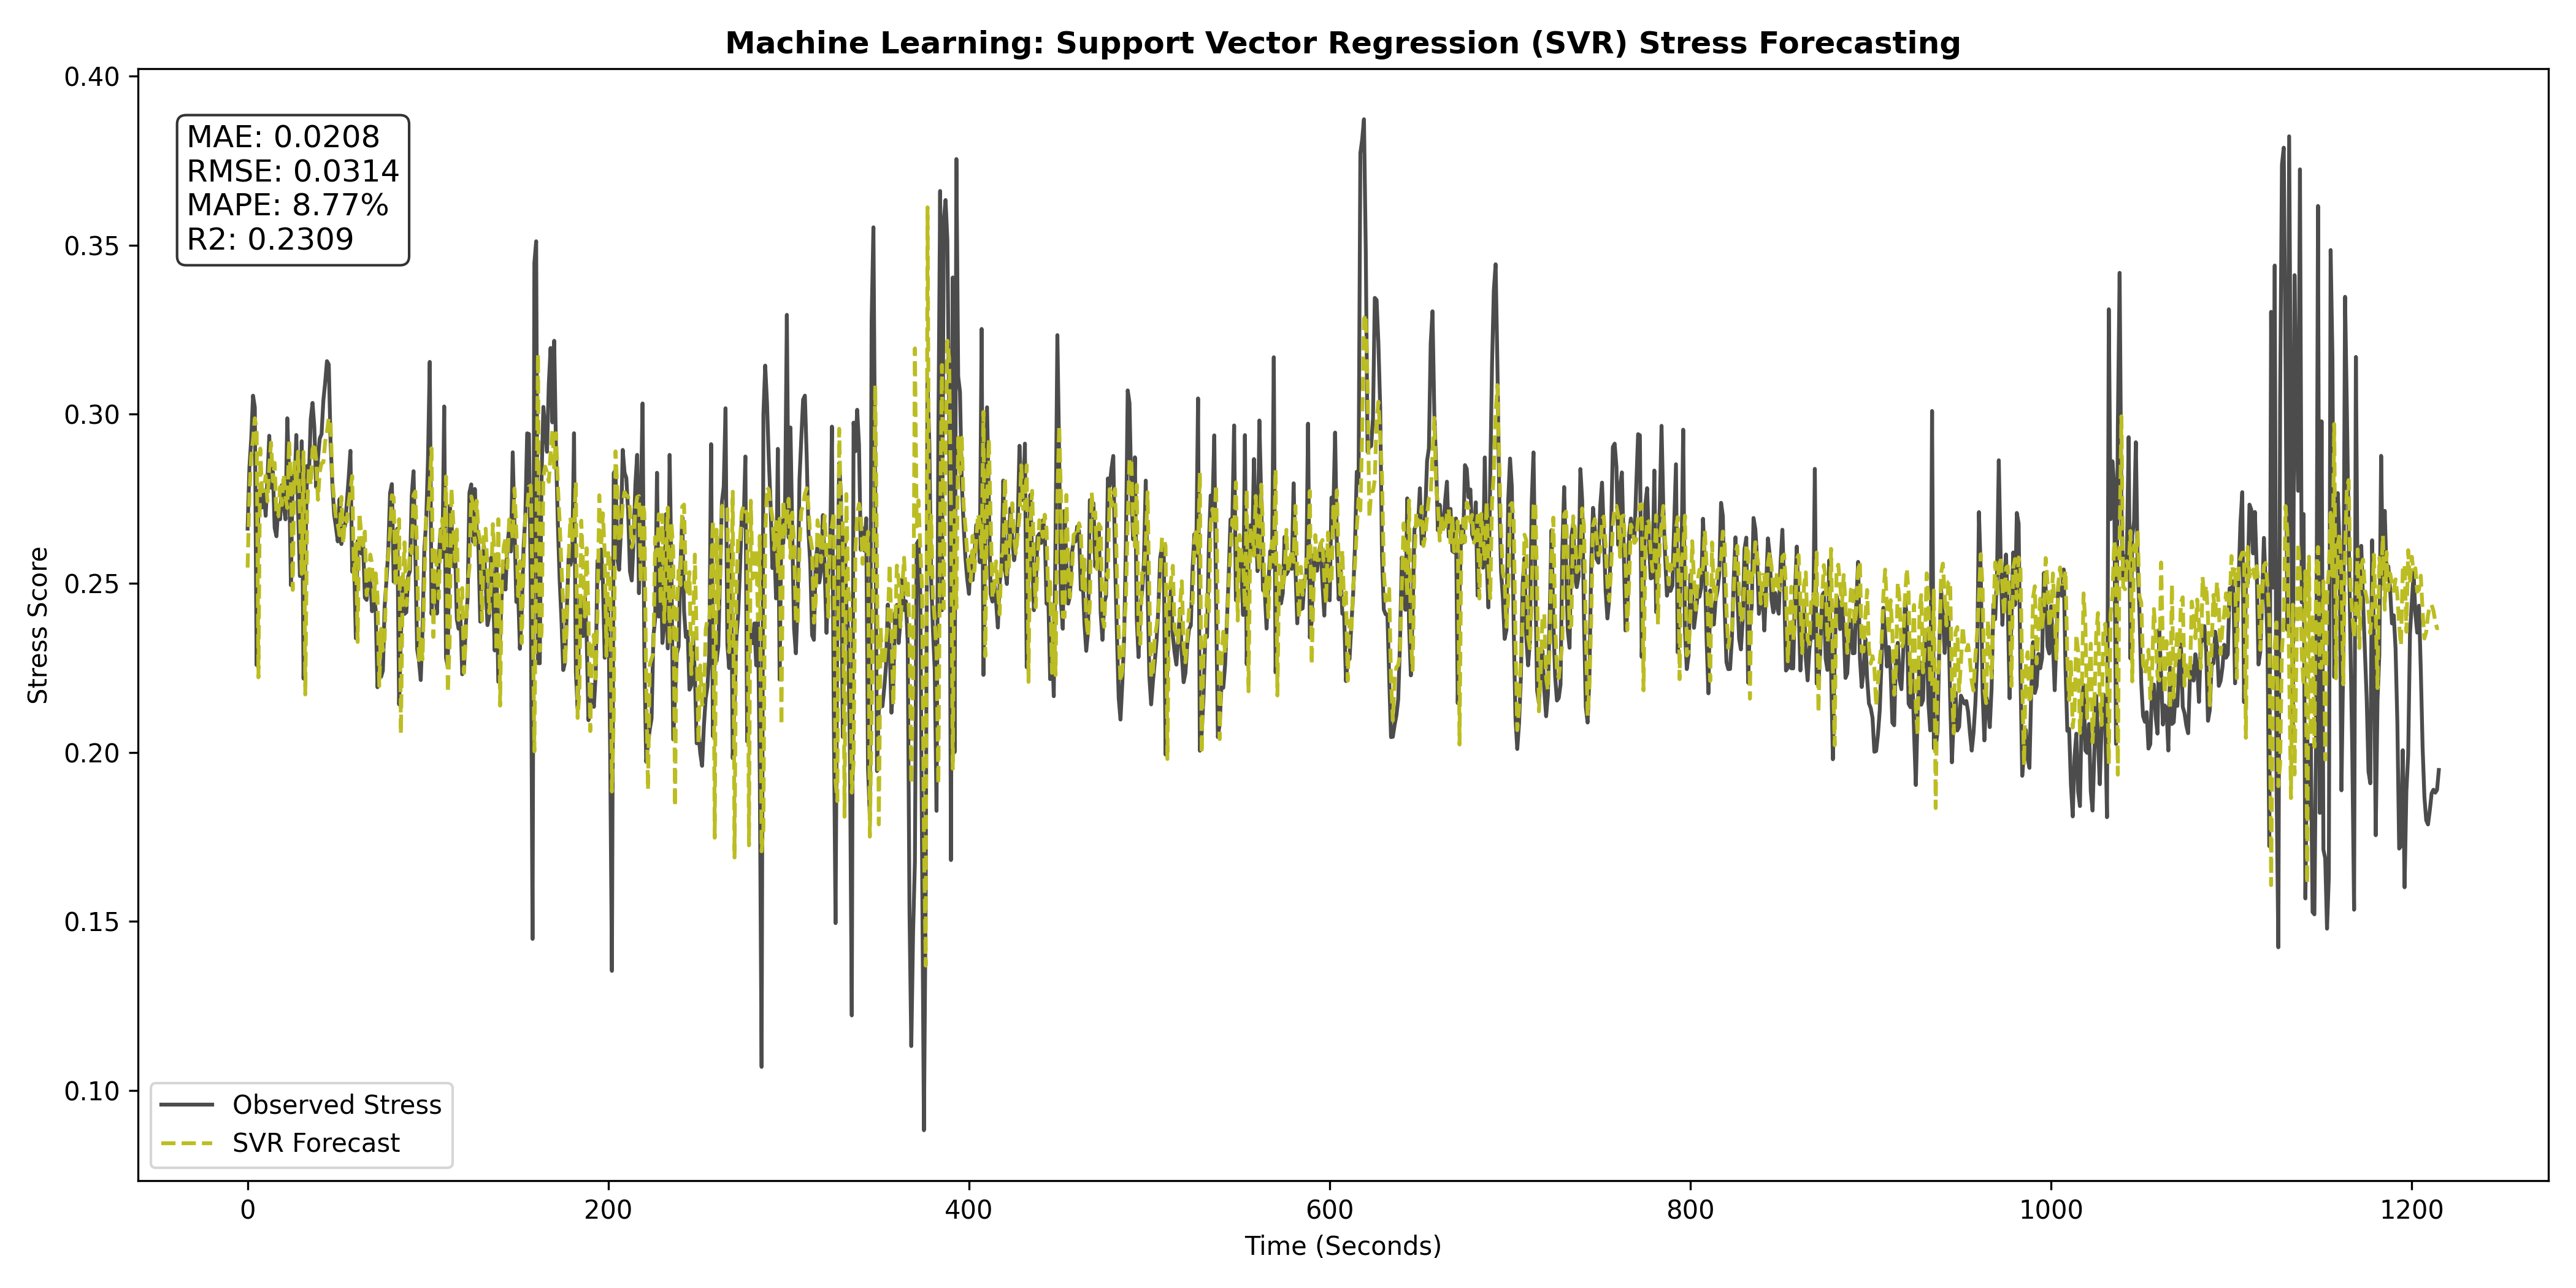
\includegraphics[width=\textwidth]{Forecasting_Graphs/11_SVR_Forecast.png} \end{column}
        \begin{column}{0.33\textwidth} \metricwidget{SVR}{0.0208}{0.0314}{8.77}{0.2309} \end{column}
    \end{columns}
\end{frame}

\begin{frame}{Model 12: GRU}
    \begin{columns}
        \begin{column}{0.65\textwidth} 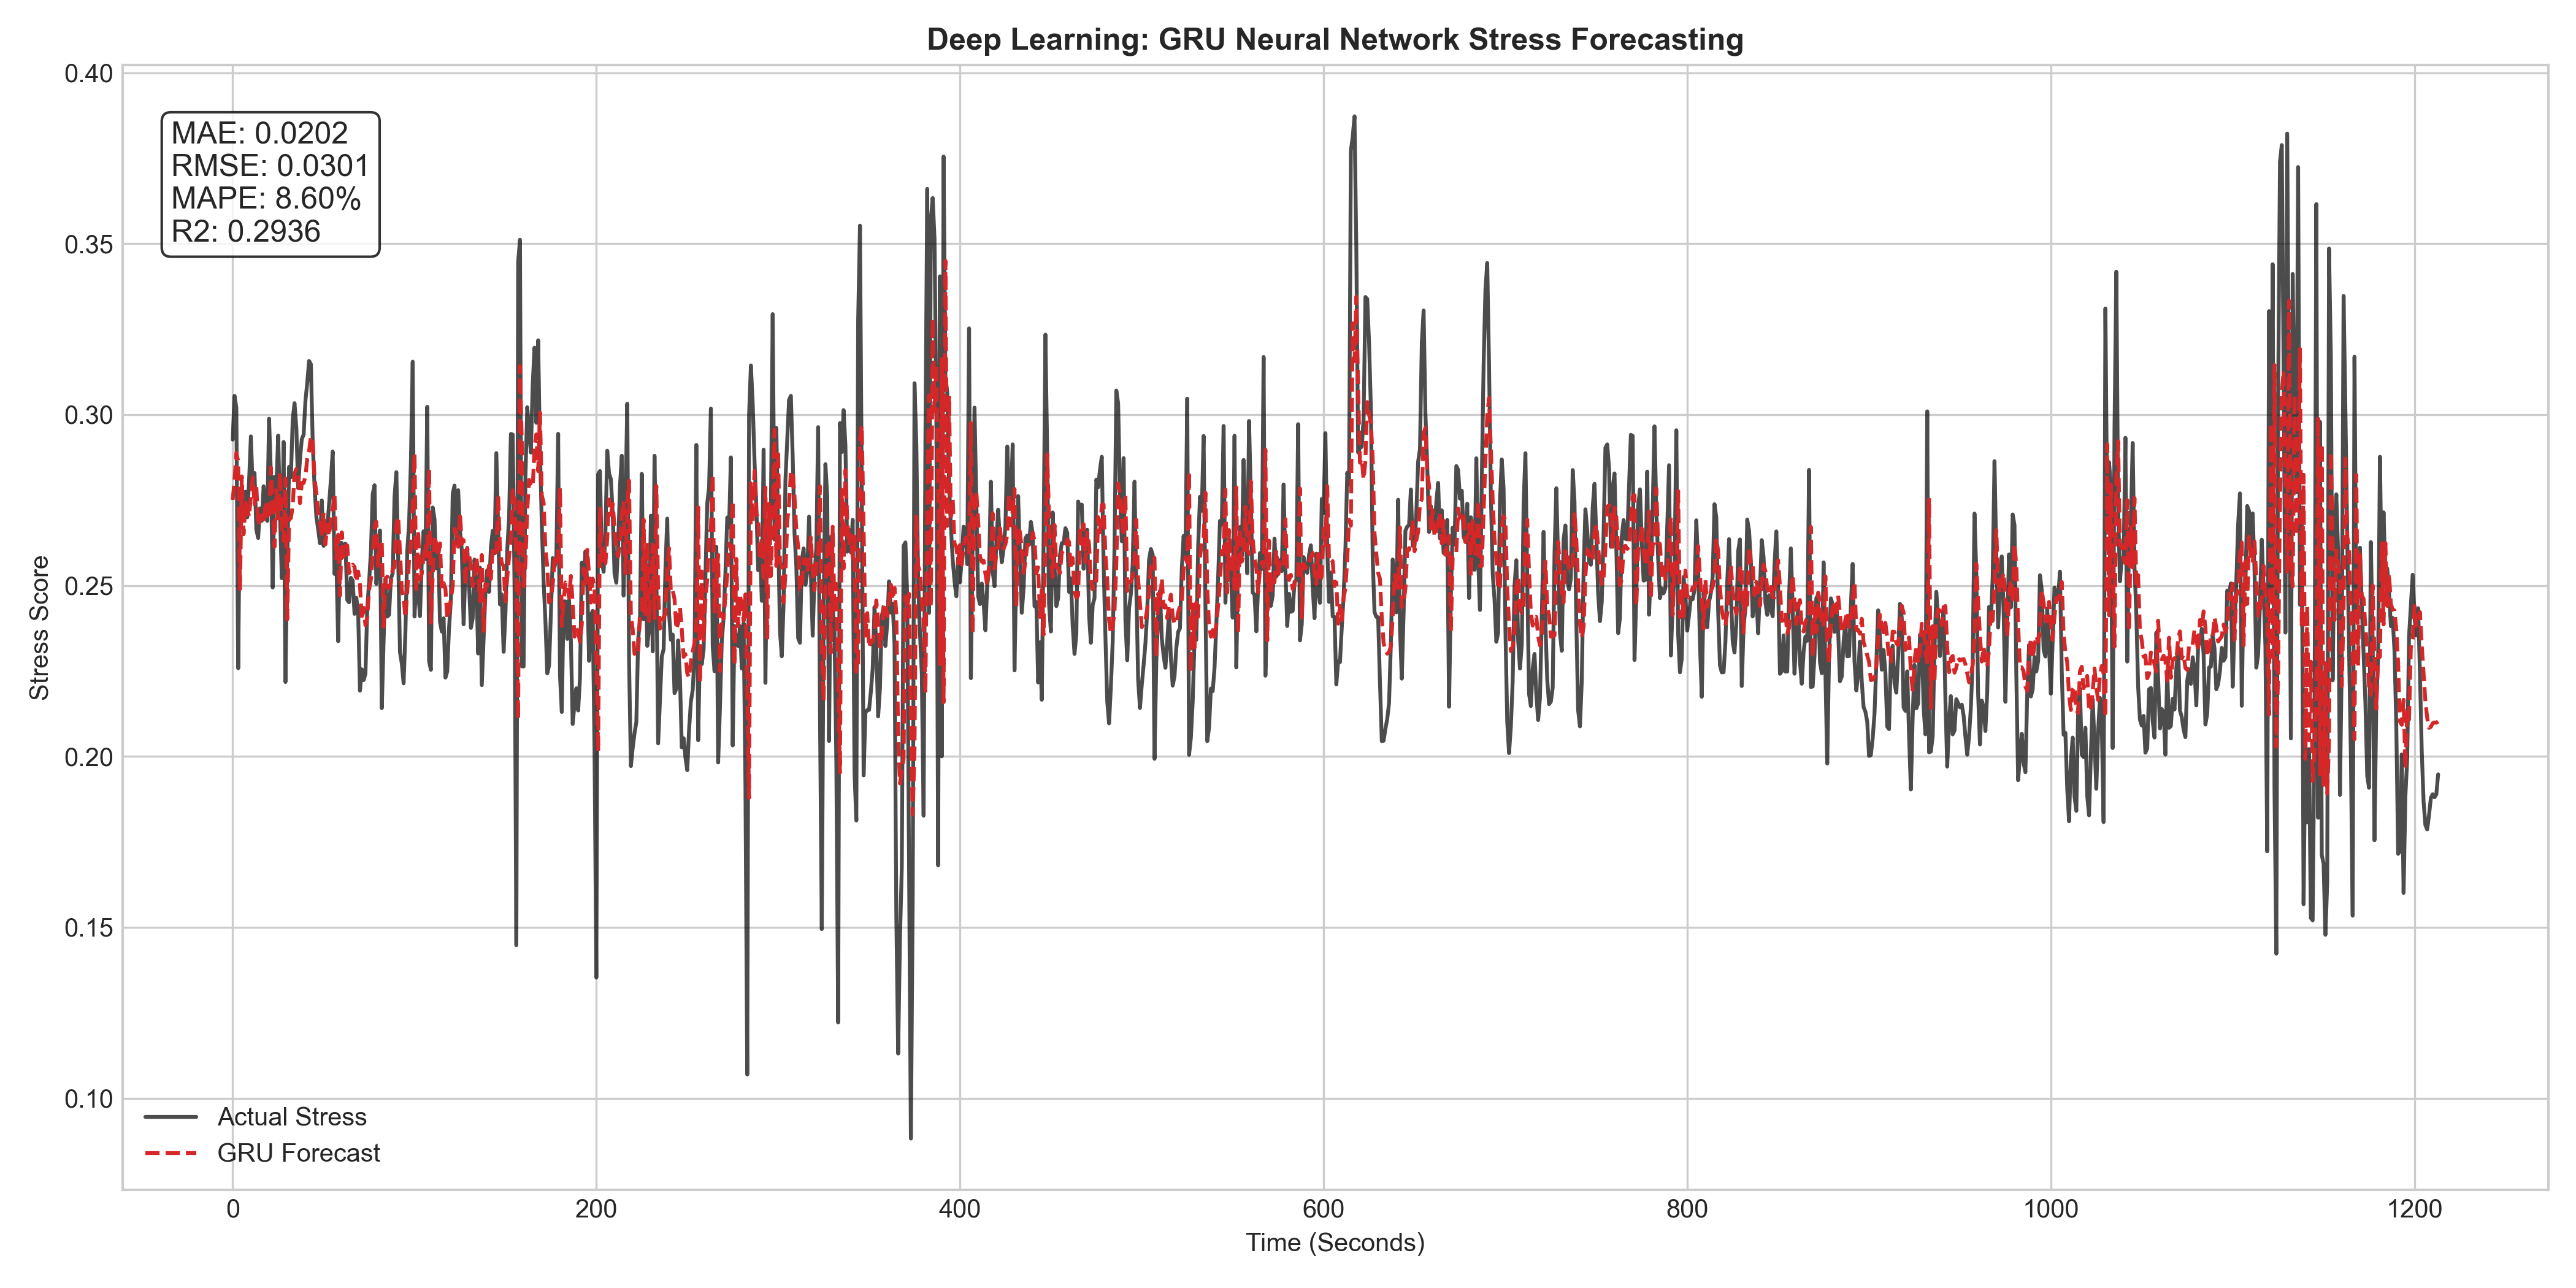
\includegraphics[width=\textwidth]{Forecasting_Graphs/12_GRU_Forecast.png} \end{column}
        \begin{column}{0.33\textwidth} \metricwidget{GRU}{0.0202}{0.0301}{8.60}{0.2936} \end{column}
    \end{columns}
\end{frame}

\begin{frame}{Model 13: Quantile Regression}
    \begin{columns}
        \begin{column}{0.65\textwidth} 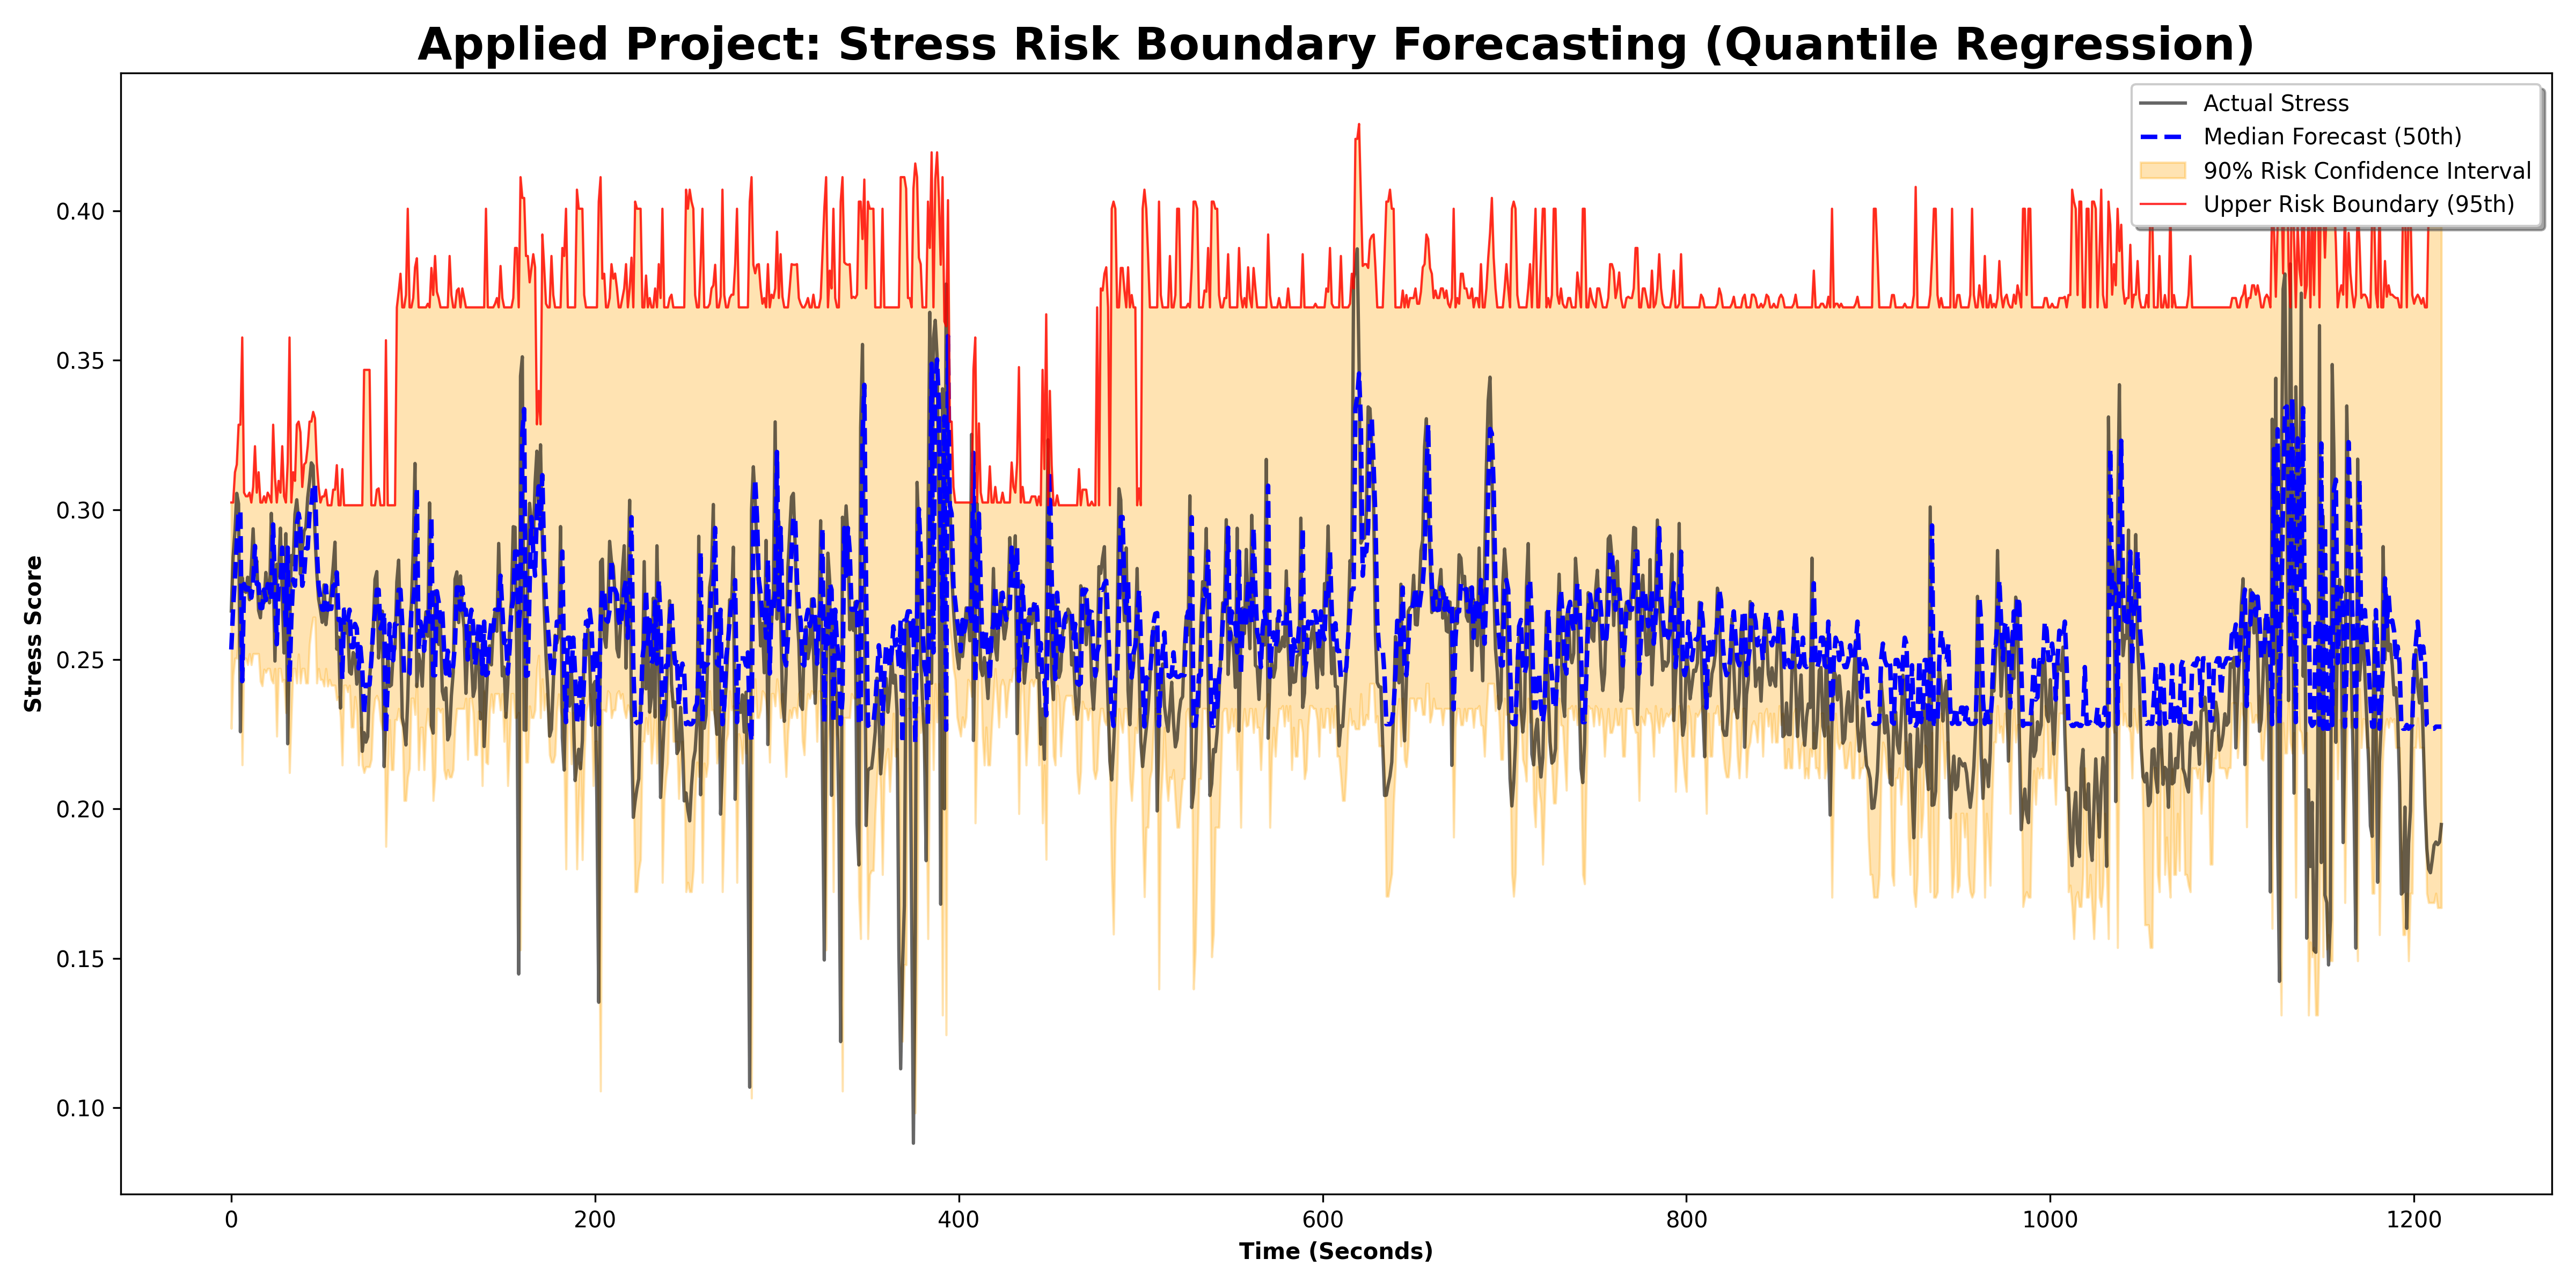
\includegraphics[width=\textwidth]{Forecasting_Graphs/13_Quantile_Risk_Boundaries.png} \end{column}
        \begin{column}{0.33\textwidth} \metricwidget{Quantile}{0.0241}{N/A}{N/A}{N/A} \end{column}
    \end{columns}
\end{frame}

\newchapter{IV}{Analytical Sensitivity Depth}
\imageslide{Feature Ablation}{EDA_Graphs/14_Feature_Ablation_Study.png}{Multivariate context achieved 2\% better accuracy than univariate baseline.}
\imageslide{Horizon Decay}{EDA_Graphs/15_Horizon_Decay_Analysis.png}{Accuracy stable up to 30s due to skin conductance inertia.}
\imageslide{Residual Analysis}{EDA_Graphs/16_Residual_Analysis.png}{Normal distribution centered at zero proves model unbiasedness.}
\imageslide{Cross-Subject Generalization}{EDA_Graphs/17_Generalization_Test.png}{S2 to S3 transfer gap confirms need for personalization.}

\newchapter{V}{Final Verdict \& Appendix}
\imageslide{Leaderboard Dashboard}{Forecasting_Graphs/99_Final_Model_Comparison.png}{Comprehensive visualization across MAE, RMSE, MAPE, and R2.}

\begin{frame}{Appendix A: Hyperparameter Tuning}
    \begin{table}[H]
        \centering \scriptsize
        \begin{tabular}{lll}
            \toprule \textbf{Model} & \textbf{Hyperparameters} & \textbf{Selection Method} \\ \midrule
            XGBoost & Learning Rate: 0.05, Estimators: 1000 & Early Stopping (50 rounds) \\
            LSTM & Hidden Units: 64, Layers: 2, Dropout: 0.1 & Validation Loss Minimization \\
            ARMA & p: 2, q: 3, d: 1 & AIC Grid Search (p:0-3, q:0-3) \\
            SVR & C: 100, Gamma: 0.1, Kernel: RBF & Standard Clinical Baseline \\
            \bottomrule
        \end{tabular}
    \end{table}
\end{frame}

\begin{frame}{Appendix B: Subject Stationarity Metrics}
    \begin{table}[H]
        \centering \small
        \begin{tabular}{lcccc}
            \toprule \textbf{Subject} & \textbf{Raw ADF} & \textbf{Raw p-val} & \textbf{Diff ADF} & \textbf{Diff p-val} \\ \midrule
            S2 (Bench) & -2.33 & 0.066 & -77.37 & \textbf{0.000} \\
            S3 & -2.10 & 0.081 & -65.20 & \textbf{0.000} \\
            S4 & -2.45 & 0.052 & -81.12 & \textbf{0.000} \\
            S10 & -2.01 & 0.112 & -72.05 & \textbf{0.000} \\
            \bottomrule
        \end{tabular}
    \end{table}
\end{frame}

\begin{frame}{Appendix C: Deep Learning Gate Mechanics}
    \begin{columns}
        \begin{column}{0.45\textwidth}
            \begin{itemize}
                \item \textbf{Forget Gate:} Decides what history to discard.
                \item \textbf{Input Gate:} Updates cell state with new EDA cues.
                \item \textbf{Output Gate:} Calculates the predicted stress score.
            \end{itemize}
        \end{column}
        \begin{column}{0.5\textwidth}
            \begin{tcolorbox}[colback=Midnight!5, colframe=Midnight, title=Mathematical Update]
                $i_t = \sigma(W_i [h_{t-1}, x_t] + b_i)$\\
                $f_t = \sigma(W_f [h_{t-1}, x_t] + b_f)$\\
                $o_t = \sigma(W_o [h_{t-1}, x_t] + b_o)$
            \end{tcolorbox}
        \end{column}
    \end{columns}
\end{frame}

\begin{frame}[plain]
    \begin{tikzpicture}[remember picture, overlay]
        \fill[Midnight] (current page.north west) rectangle (current page.south east);
        \node[anchor=center, white, font=\huge\bfseries] at (current page.center) {THANK YOU};
    \end{tikzpicture}
\end{frame}

\end{document}
